% A LaTeX template for MSc Thesis submissions to 
% Politecnico di Milano (PoliMi) - School of Industrial and Information Engineering
%
% S. Bonetti, A. Gruttadauria, G. Mescolini, A. Zingaro
% e-mail: template-tesi-ingind@polimi.it
%
% Last Revision: October 2021
%
% Copyright 2021 Politecnico di Milano, Italy. NC-BY

\documentclass{Configuration_Files/PoliMi3i_thesis}

%------------------------------------------------------------------------------
%	REQUIRED PACKAGES AND  CONFIGURATIONS
%------------------------------------------------------------------------------

% CONFIGURATIONS
\usepackage{parskip} % For paragraph layout
\usepackage{setspace} % For using single or double spacing
\usepackage{emptypage} % To insert empty pages
\usepackage{multicol} % To write in multiple columns (executive summary)
\usepackage{multirow}
\setlength\columnsep{15pt} % Column separation in executive summary
\setlength\parindent{0pt} % Indentation
\raggedbottom  

% PACKAGES FOR TITLES
\usepackage{titlesec}
% \titlespacing{\section}{left spacing}{before spacing}{after spacing}
\titlespacing{\section}{0pt}{3.3ex}{2ex}
\titlespacing{\subsection}{0pt}{3.3ex}{1.65ex}
\titlespacing{\subsubsection}{0pt}{3.3ex}{1ex}
\usepackage{color}

% PACKAGES FOR LANGUAGE AND FONT
\usepackage[english]{babel} % The document is in English  
\usepackage[utf8]{inputenc} % UTF8 encoding
\usepackage[T1]{fontenc} % Font encoding
\usepackage[11pt]{moresize} % Big fonts

% PACKAGES FOR IMAGES
\usepackage{graphicx}
\usepackage{transparent} % Enables transparent images
\usepackage{eso-pic} % For the background picture on the title page
\usepackage{subfig} % Numbered and caption subfigures using \subfloat.
\usepackage{tikz} % A package for high-quality hand-made figures.
\usetikzlibrary{}
\graphicspath{{./Images/}} % Directory of the images
\usepackage{caption} % Coloured captions
\usepackage{xcolor} % Coloured captions
\usepackage{amsthm,thmtools,xcolor} % Coloured "Theorem"
\usepackage{float}

% STANDARD MATH PACKAGES
\usepackage{amsmath}
\usepackage{amsthm}
\usepackage{amssymb}
\usepackage{amsfonts}
\usepackage{bm}
\usepackage[overload]{empheq} % For braced-style systems of equations.
\usepackage{fix-cm} % To override original LaTeX restrictions on sizes

% PACKAGES FOR TABLES
\usepackage{tabularx}
\usepackage{longtable} % Tables that can span several pages
\usepackage{colortbl}

% PACKAGES FOR ALGORITHMS (PSEUDO-CODE)
\usepackage{algorithm}
\usepackage{algorithmic}

% PACKAGES FOR REFERENCES & BIBLIOGRAPHY
\usepackage[colorlinks=true,linkcolor=black,anchorcolor=black,citecolor=black,filecolor=black,menucolor=black,runcolor=black,urlcolor=black]{hyperref} % Adds clickable links at references
\usepackage{cleveref}
\usepackage[square, numbers, sort&compress]{natbib} % Square brackets, citing references with numbers, citations sorted by appearance in the text and compressed
\bibliographystyle{abbrvnat} % You may use a different style adapted to your field

% OTHER PACKAGES
\usepackage{pdfpages} % To include a pdf file
\usepackage{afterpage}
\usepackage{lipsum} % DUMMY PACKAGE
\usepackage{fancyhdr} % For the headers
\usepackage{enumitem}
\fancyhf{}

% Input of configuration file. Do not change config.tex file unless you really know what you are doing. 
% Define blue color typical of polimi
\definecolor{bluepoli}{cmyk}{0.4,0.1,0,0.4}

% Custom theorem environments
\declaretheoremstyle[
  headfont=\color{bluepoli}\normalfont\bfseries,
  bodyfont=\color{black}\normalfont\itshape,
]{colored}

% Set-up caption colors
\captionsetup[figure]{labelfont={color=bluepoli}} % Set colour of the captions
\captionsetup[table]{labelfont={color=bluepoli}} % Set colour of the captions
\captionsetup[algorithm]{labelfont={color=bluepoli}} % Set colour of the captions

\theoremstyle{colored}
\newtheorem{theorem}{Theorem}[chapter]
\newtheorem{proposition}{Proposition}[chapter]

% Enhances the features of the standard "table" and "tabular" environments.
\newcommand\T{\rule{0pt}{2.6ex}}
\newcommand\B{\rule[-1.2ex]{0pt}{0pt}}

% Pseudo-code algorithm descriptions.
\newcounter{algsubstate}
\renewcommand{\thealgsubstate}{\alph{algsubstate}}
\newenvironment{algsubstates}
  {\setcounter{algsubstate}{0}%
   \renewcommand{\STATE}{%
     \stepcounter{algsubstate}%
     \Statex {\small\thealgsubstate:}\space}}
  {}

% New font size
\newcommand\numfontsize{\@setfontsize\Huge{200}{60}}

% Title format: chapter
\titleformat{\chapter}[hang]{
\fontsize{50}{20}\selectfont\bfseries\filright}{\textcolor{bluepoli} \thechapter\hsp\hspace{2mm}\textcolor{bluepoli}{|   }\hsp}{0pt}{\huge\bfseries \textcolor{bluepoli}
}

% Title format: section
\titleformat{\section}
{\color{bluepoli}\normalfont\Large\bfseries}
{\color{bluepoli}\thesection.}{1em}{}

% Title format: subsection
\titleformat{\subsection}
{\color{bluepoli}\normalfont\large\bfseries}
{\color{bluepoli}\thesubsection.}{1em}{}

% Title format: subsubsection
\titleformat{\subsubsection}
{\color{bluepoli}\normalfont\large\bfseries}
{\color{bluepoli}\thesubsubsection.}{1em}{}

% Shortening for setting no horizontal-spacing
\newcommand{\hsp}{\hspace{0pt}}

\makeatletter
% Renewcommand: cleardoublepage including the background pic
\renewcommand*\cleardoublepage{%
  \clearpage\if@twoside\ifodd\c@page\else
  \null
  \AddToShipoutPicture*{\BackgroundPic}
  \thispagestyle{empty}%
  \newpage
  \if@twocolumn\hbox{}\newpage\fi\fi\fi}
\makeatother

%For correctly numbering algorithms
\numberwithin{algorithm}{chapter}

%----------------------------------------------------------------------------
%	NEW COMMANDS DEFINED
%----------------------------------------------------------------------------

% EXAMPLES OF NEW COMMANDS
\newcommand{\bea}{\begin{eqnarray}} % Shortcut for equation arrays
\newcommand{\eea}{\end{eqnarray}}
\newcommand{\e}[1]{\times 10^{#1}}  % Powers of 10 notation

%----------------------------------------------------------------------------
%	ADD YOUR PACKAGES (be careful of package interaction)
%----------------------------------------------------------------------------

%----------------------------------------------------------------------------
%	ADD YOUR DEFINITIONS AND COMMANDS (be careful of existing commands)
%----------------------------------------------------------------------------

%----------------------------------------------------------------------------
%	BEGIN OF YOUR DOCUMENT
%----------------------------------------------------------------------------

\begin{document}

\fancypagestyle{plain}{%
\fancyhf{} % Clear all header and footer fields
\fancyhead[RO,RE]{\thepage} %RO=right odd, RE=right even
\renewcommand{\headrulewidth}{0pt}
\renewcommand{\footrulewidth}{0pt}}

%----------------------------------------------------------------------------
%	TITLE PAGE
%----------------------------------------------------------------------------

\pagestyle{empty} % No page numbers
\frontmatter % Use roman page numbering style (i, ii, iii, iv...) for the preamble pages

\puttitle{
	title=Design Document, % Title of the thesis
	name=Conti Enzo and Marino María, % Author Name and Surname
	course=Computer Science and Engineering, % Study Programme (in Italian)
	academicyear={2024-25},  % Academic Year
} % These info will be put into your Title page 

%----------------------------------------------------------------------------
%	PREAMBLE PAGES: ABSTRACT (inglese e italiano), EXECUTIVE SUMMARY
%----------------------------------------------------------------------------
\startpreamble
\setcounter{page}{1} % Set page counter to 1

%----------------------------------------------------------------------------
%	LIST OF CONTENTS/FIGURES/TABLES/SYMBOLS
%----------------------------------------------------------------------------

% TABLE OF CONTENTS
\thispagestyle{empty}
\tableofcontents % Table of contents 
\thispagestyle{empty}
\cleardoublepage

%-------------------------------------------------------------------------
%	THESIS MAIN TEXT
%-------------------------------------------------------------------------
% In the main text of your thesis you can write the chapters in two different ways:
%
%(1) As presented in this template you can write:
%    \chapter{Title of the chapter}
%    *body of the chapter*
%
%(2) You can write your chapter in a separated .tex file and then include it in the main file with the following command:
%    \chapter{Title of the chapter}
%    \input{chapter_file.tex}
%
% Especially for long thesis, we recommend you the second option.

\addtocontents{toc}{\vspace{2em}} % Add a gap in the Contents, for aesthetics
\mainmatter % Begin numeric (1,2,3...) page numbering

% --------------------------------------------------------------------------
% NUMBERED CHAPTERS % Regular chapters following
% --------------------------------------------------------------------------
\chapter{Introduction}
\label{ch:introduction}%
\section{Purpose}
As the demand for skilled professionals grows, facilitating smooth connections between students and companies becomes increasingly vital. Traditionally, students seeking internships often face challenges in finding opportunities that align with their skills and career goals, while companies struggle to identify the right talent. The Students\&Companies (S\&C) platform addresses this challenge by providing a space where university students and companies offering internships can easily find and connect with each other.

S\&C simplifies the process by matching students with internships based on their skills, experiences, and the opportunities offered by companies. The platform enhances the internship search and recruitment process, making it more efficient for both students looking to gain real-world experience and companies seeking fresh talent. By fostering better connections and streamlining communication, S\&C helps ensure that both students and companies can find the right fit, ultimately benefiting the growth of the workforce.
\section{Scope}
In this section, we define the domain of the Students\&Companies (S\&C) platform, focusing on the main users and their interactions with the system. There are two primary user groups: Students and Companies.

Students are individuals enrolled in universities who use the platform to search for and apply to internship opportunities. They can create and manage their profiles, upload their CVs, and receive recommendations for internships that match their skills and preferences. Students can also proactively browse available internships, apply to them, and track the status of their applications.

Companies are organizations offering internships, using the platform to advertise available opportunities. They can post detailed internship descriptions, including tasks, benefits, and the skills required. Companies can also review student profiles, receive recommendations, and initiate the selection process, which may involve interviews and other assessments.

The platform facilitates a two-way interaction: students receive recommendations for internships that align with their qualifications, and companies can identify and reach out to students who fit their needs. Both students and companies can track the progress of their applications or listings and provide feedback to improve the matching process. Additionally, universities are involved in monitoring the internships, ensuring quality, and supporting students throughout the experience.
\section{Definitions, Acronyms, Abbreviations}
\begin{itemize}
    \item S\&C Students\&Companies
    \item UI User Interface
    \item RASD Requirement Analysis and Specification Document
    \item DD Design Document
    \item HTTPS/REST The usage of a Representational State Transfer API to commuicate using the HyperText Transfer Protocol Secure protocol
\end{itemize}
\section{Revision history}
Version 1.0 (30/12/2024)
\section{Reference Documents}
This document is based on the following materials
\begin{itemize}
    \item R\&DD assignment specification of the Software Engineering II course a.a. 2024/5
    \item Slides of the same course available on WeBeep
\end{itemize}
\section{Document Structure}
\begin{itemize}
  \item \textbf{Introduction:} In this section we introduce the project and the Design Document.
  \item \textbf{Architectural Design:} This section describes in detail the architecture selected for the project.
  \item \textbf{User Interface Design:} In this section we show some prototypes of the user interface that aim to showcase the look and feel of the platform.
  \item \textbf{ Requirements Traceability:} In this section the requirements defined in the RASD are mapped to the different components defined in this document.
  \item \textbf{Implementation, Integration and Test Plan:} In this section we define the implementation and testing plans, providing a rationale for each.
  \item \textbf{Effort Spent:} Time spent on each section of the document.
  \item \textbf{References:} List of documents and software references used in the paper.
  \end{itemize}




\chapter{Architectural Design}
\label{ch:architectural_design}%
\section{Overview} 

\begin{figure}[H]
    \centering
    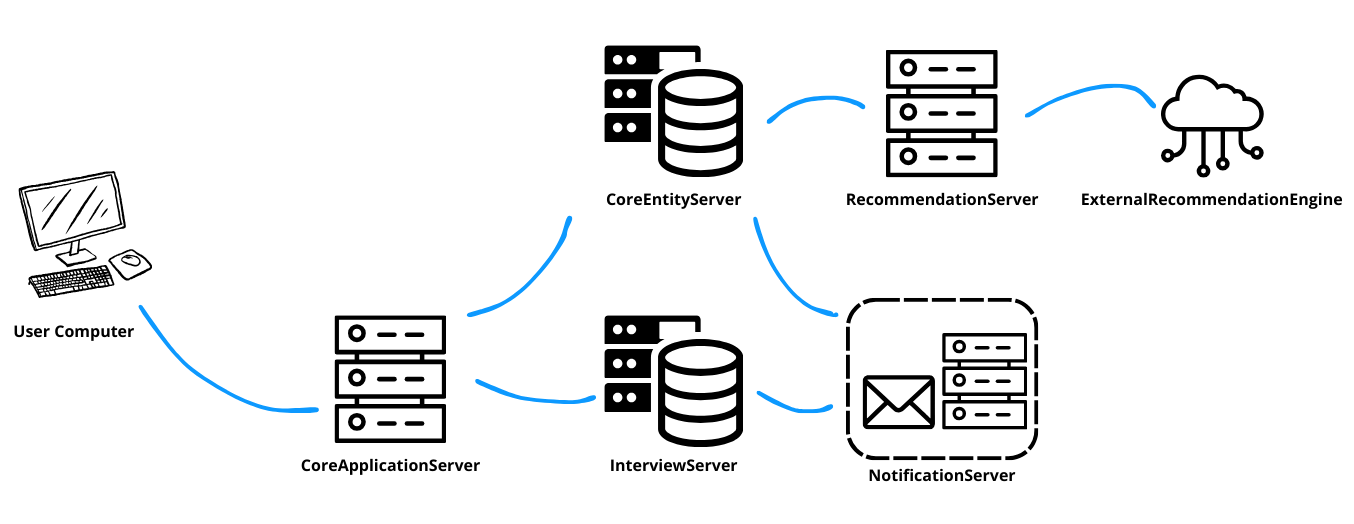
\includegraphics[width=\textwidth]{Images/informal-view.png}
    \caption{Informal View of the System}
    \label{fig:informal_view}
\end{figure}

The informal view of the system provides a high-level representation of the key components and their interactions within the Students\&Companies (S\&C) platform. The design prioritizes modularity, scalability, and maintainability, reflecting the architectural decisions made to address the platform's requirements effectively.

A microservices architecture forms the foundation of the system, enabling decoupled services to interact through well-defined interfaces. This design choice ensures that individual components, such as authentication, matchmaking, and notifications, can be developed, deployed, and scaled independently. Communication between these components is facilitated through secure RESTful APIs and asynchronous messaging systems, enhancing fault tolerance and performance.

By abstracting critical elements like the RecommendationEngine as a black-box component, the design provides flexibility for future updates or replacements without disrupting other parts of the system. Furthermore, distributed databases ensure data consistency and fault isolation, allowing the platform to handle a diverse range of user interactions efficiently.


\section{Component view}

As mentioned, the chosen architecture is a microservice architecture, in which the components are abstracted to include a decoupled service and they interact with each other with well defined interfaces to request for each others different competences. The component view can be seen at \ref{fig:component_diagram} and describes the following components:
\begin{itemize}
    \item \textbf{AuthenticationService} provides the authentication of user credentials
    \item \textbf{Main Platform} routes the API calls from the FrontEndInterface to other components with respective databases and services, also takes part in coordination in some use cases.
    \item \textbf{FrontEndInterface} is the graphic user interface available to the user through Web
    \item \textbf{HistoryManager} is responsible for storing and maintaining complaints and feedbacks of users.
    \item \textbf{CoreEntityManager} is responsible for storing, mantaining and giving functionality to some core entities, such as internships, students, applications, etc.
    \item \textbf{InterviewManager} is strictly responsible to store, maintain and give the functionalities of interview, including start it, finish it, assess its handling by the company user etc.
    \item \textbf{RecommendationScheduler} is responsible to periodically scan for reccomendations and coordinate the handling of the recommendation engine
    \item \textbf{DataProcessor} is responsible to assess RecommendationScheduler and CoreEntityManager on the data cleaning and pre processing to send to the RecommendationEngine
    \item \textbf{RecomendationEngine} models the external cloud tool to generate recommendations for internships and students
    \item \textbf{NotificationListener} is responsible of taking in messages of entities that wish to send notifications to actors
    \item \textbf{NotificationDispatcher} is responsible to receive the notification requests and dispatch it to the users through a mailing service, also includes in its internal logic choices as in how often to email etc.

    
    
\end{itemize}

\begin{figure}[H]
    \centering
    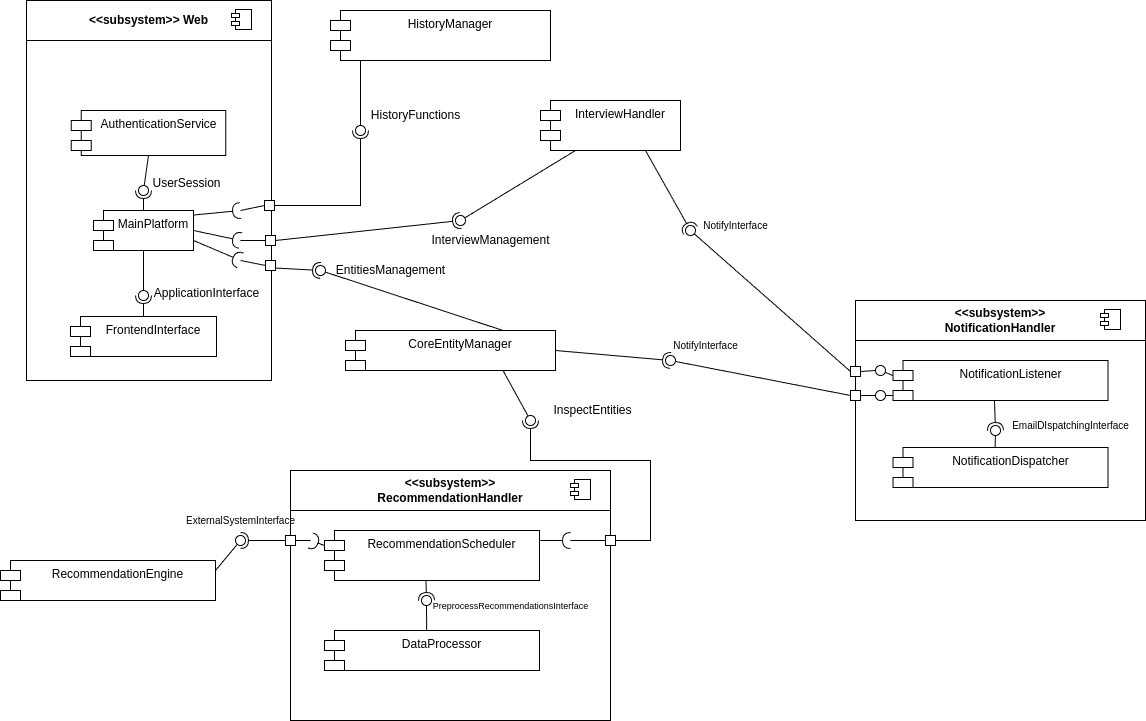
\includegraphics[width=\textwidth]{Images/component-view.png}
    \caption{Component Diagram}
    \label{fig:component_diagram}
\end{figure}

\section{Deployment view}

Here is shown the deployment view diagram, which is important because it illustrates the physical layout of the system, showing how software components are deployed onto hardware nodes. This view is essential for understanding system scalability, fault tolerance, and performance optimization by highlighting the relationships and communication paths between components. It can be seen on figure \ref{fig:deployment_diagram}.

\begin{figure}[H]
    \centering
    \rotatebox{90}{
        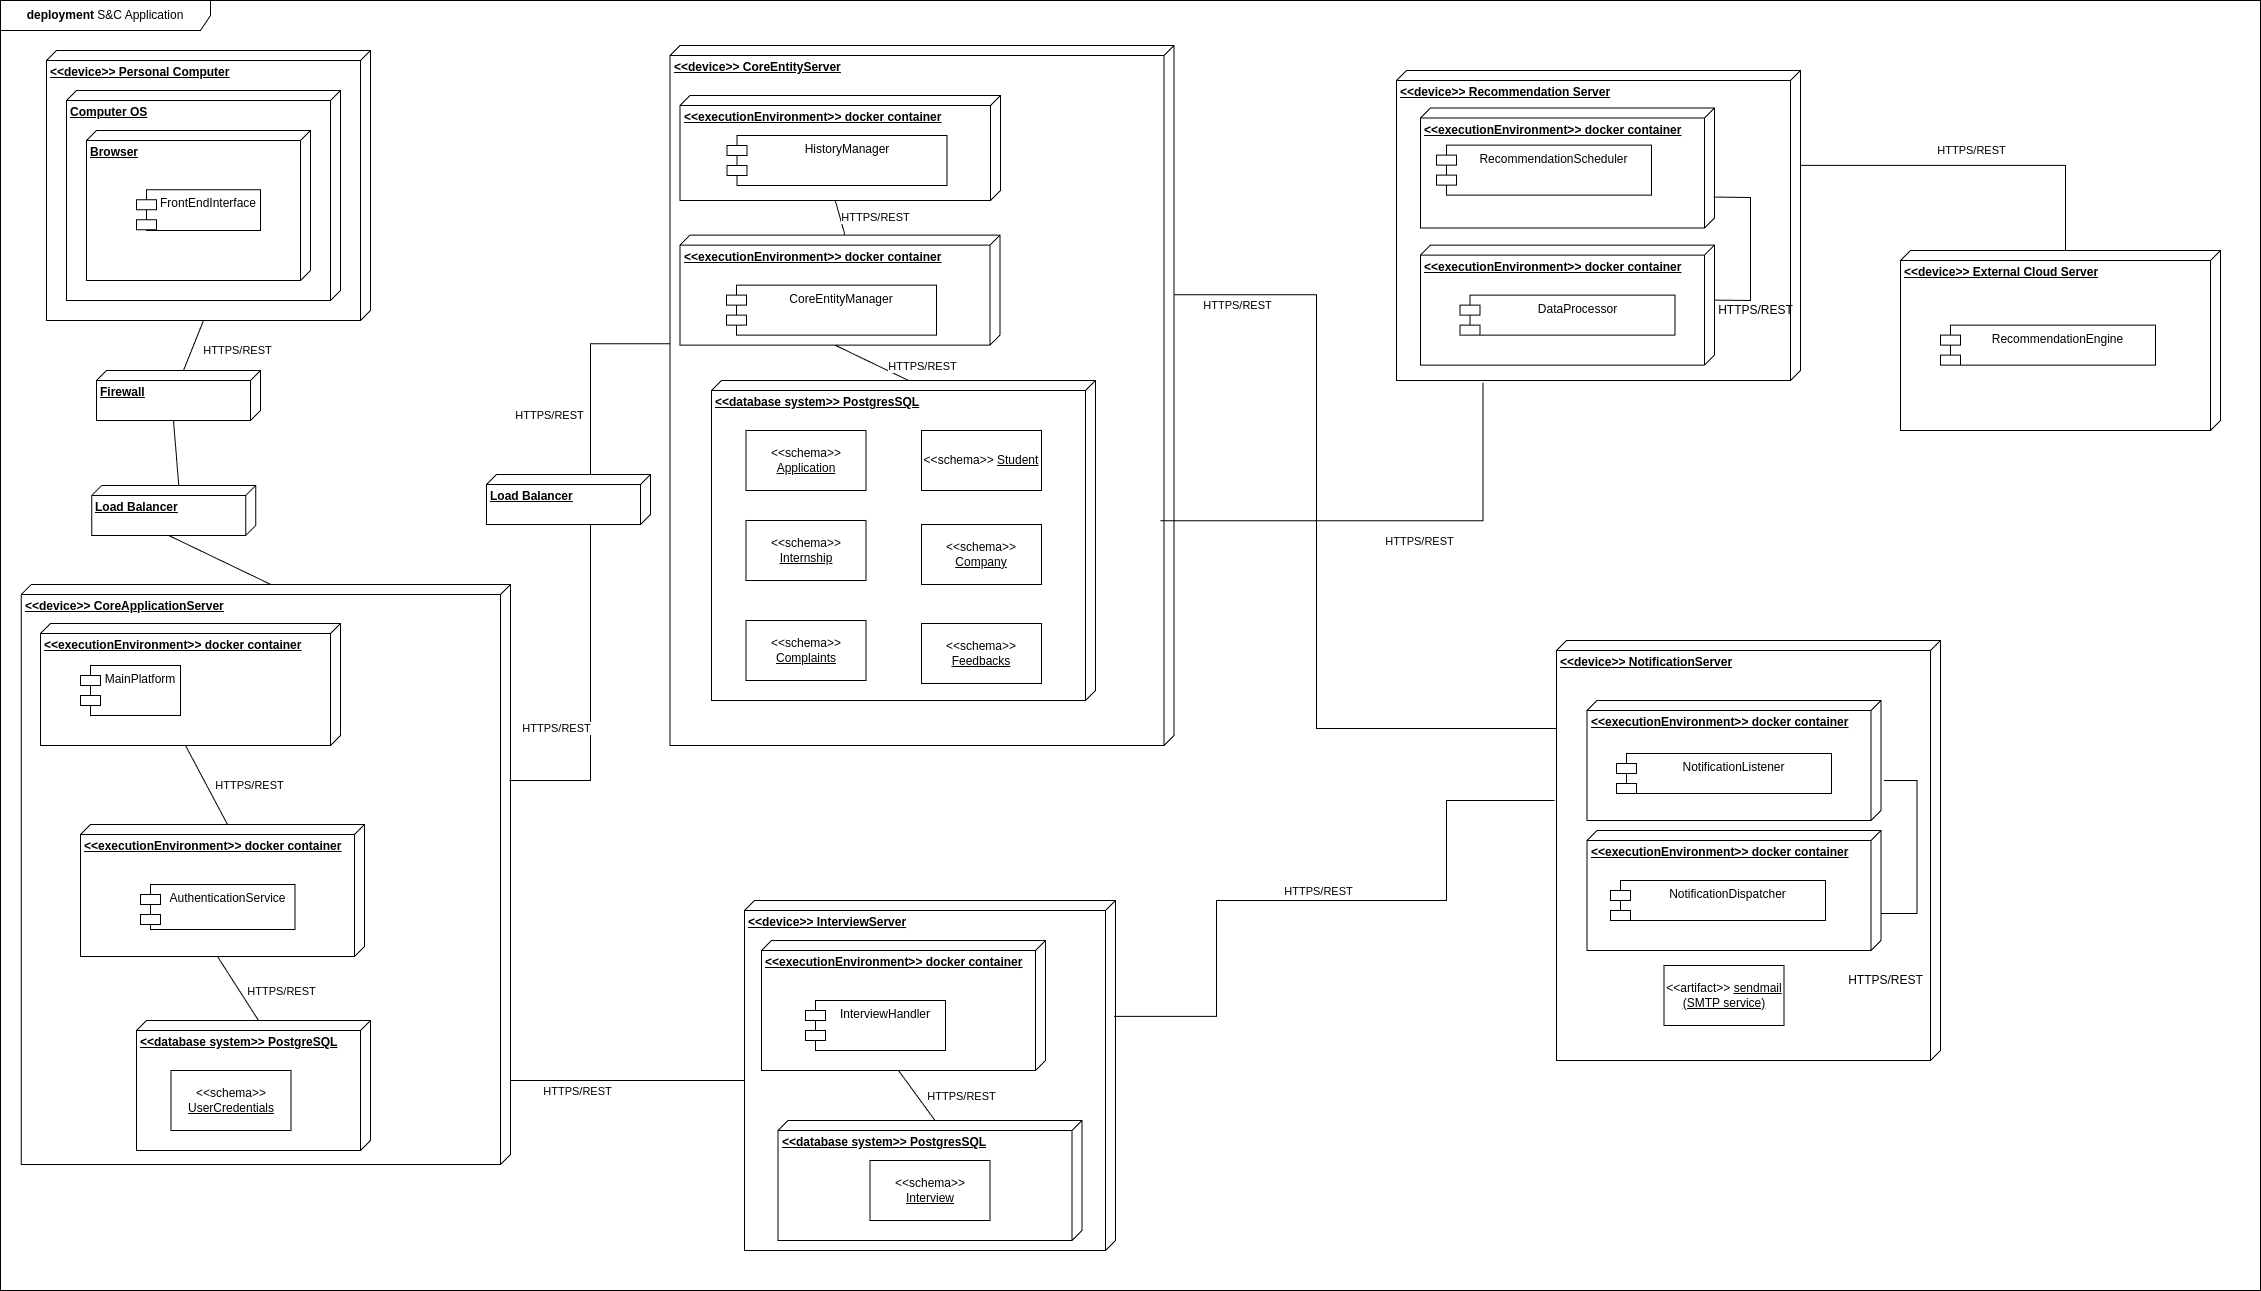
\includegraphics[width=0.9\textheight]{Images/deployment-view.png}
    }
    \caption{Specification Level Deployment Diagram}
    \label{fig:deployment_diagram}
\end{figure}

In \ref{fig:deployment_diagram} it can be seen that the microservices architecture allows a distributed implementation onto hardware which can be exploited also for replication and optimization, achieving reliabilty, safety and secureness, and fault tolerance.
The components are all abstracted on a docker container so that the system is portable and the architecture can change without major firmware issues. Also, the components are grouped in different servers according to functionality and frequency of communication.

The LoadBalancers guarantee that replicated critical servers and components have a reasonably equal workload among them, and the firewall protects against attacks comming from the FrontEndInterface, which is runned on the browser of the user and therefore we have less control of. The NotificationServer also includes a mailing system so that the NotificationDispatcher can send emails via SMTP, and the RecommendationEngine is modelled as an external server running on a cloud solution. 

All servers communicate through HTTPS/REST API calls defined internally on the system, except the RecommendationEngine that is defined by the solution itself, but the RecommendationServer components adress this internally.

\section{Runtime view}

This section introduces the runtime view of the system, that is, its dynamic behavior across use cases. The 4 use cases that were documented on the RASD with sequence diagrams also have their sequence diagrams here for coherence with the RASD, while the other simpler ones are explained textually.

\textbf{[UC1] Form Filling}

The user fills the empty form on the FrontEndInterface and submits it. The FrontEndInterface sends the data to the MainPlatform, which runs its validation logic. In case of validation failure, an error is returned to the FrontEndInterface for user correction. Here, the MainPlatform can apply some other procedures on the data (for example, send it to other component for storage). Finally, the MainPlatform sends an ``OK'' back to the FrontEndInterface, which displays a success message.


\textbf{[UC2] Register Student}

The student opens the S\&C Website via the FrontEndInterface and clicks ``New Account''. The FrontEndInterface requests a registration form from the MainPlatform, which calls the AuthenticationService to validate and store the new user’s credentials. Meanwhile, any additional profile information is passed from the MainPlatform to the CoreEntityManager for storage. Once validation succeeds, both the AuthenticationService and CoreEntityManager send ``OK'' back to the MainPlatform, which then notifies the FrontEndInterface. Finally, the FrontEndInterface displays a confirmation that the student’s account is successfully registered.

\textbf{[UC3] Register Company}

The company employee opens the S\&C Website via the FrontEndInterface and clicks ``New Account''. The FrontEndInterface requests a registration form from the MainPlatform, which calls the AuthenticationService to validate and store the new company account credentials (email, password). Meanwhile, any additional company data (e.g., name, industry) is passed from the MainPlatform to the CoreEntityManager for storage. Once both the AuthenticationService and CoreEntityManager send an ``OK'' back to the MainPlatform, the MainPlatform notifies the FrontEndInterface. Finally, the FrontEndInterface displays a confirmation that the company account has been successfully created.

\textbf{[UC4] User Login}

The user opens the S\&C Website on the FrontEndInterface and clicks ``Log In''. The FrontEndInterface sends the entered email and password to the MainPlatform, which calls the AuthenticationService to check the credentials. If valid, the AuthenticationService confirms, and the MainPlatform creates a user session. It then notifies the FrontEndInterface, which displays the user’s dashboard. If invalid, the MainPlatform returns an error message, leading the FrontEndInterface to prompt the user to retry.


\textbf{[UC5] Search Internship} (Figure \ref{fig:searchsequence})
\begin{figure}[H]
\centering
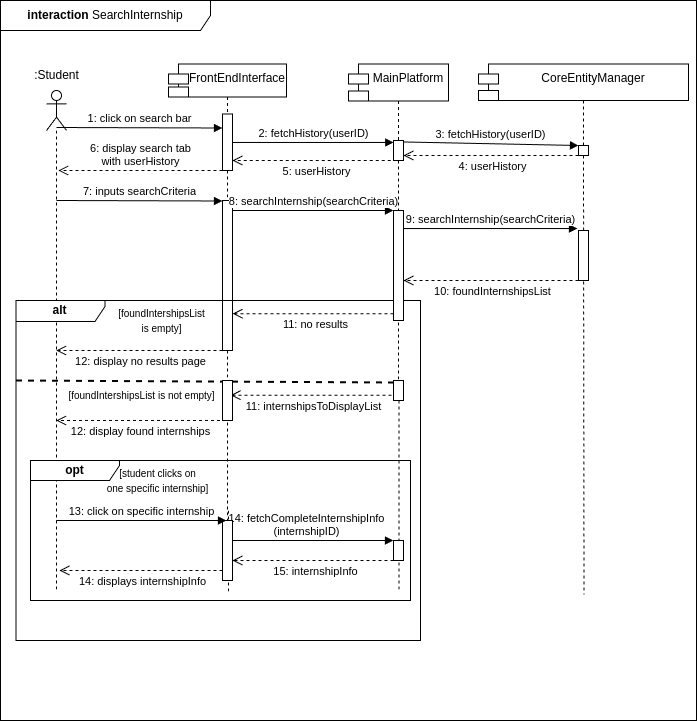
\includegraphics[width=\textwidth]{Images/search-internship-sequence.png}
\caption{\label{fig:searchsequence} Search Internship Sequence Diagram}
\end{figure}


The process is started when a Student clicks on the Search Bar once in the main page, which makes the FrontEndInterface fetch the userHistory of that user to display the beneath the search bar. With the history displayed, the Student inputs the desired search criteria on the FrontEndInterface or picks from his recent history, which passes it to the MainPlatform, that also passes it to the CoreEntityManager. This component then looks up on its internal database and passes back to the MainPlatform, which returns with either a ``no result'' to the FrontEndInterface or the list of found internships, depending on this list being empty or not.

Once the results are showed, if any, the student may click on a specific internship, causing the FrontEndInterface to fetch the remaining information of the internship from the MainPlatform (cached after the first fetch) and, after response, the user can see it.

\textbf{[UC6] Apply Internship}

The student, already logged in, views the internship details through the FrontEndInterface. When they click the ``Apply'' button, the FrontEndInterface sends the application request to the MainPlatform, which recognizes the active user session. The MainPlatform then forwards this request to the CoreEntityManager to record the application. Once saved, the CoreEntityManager confirms back to the MainPlatform, which returns a success status to the FrontEndInterface. Finally, the FrontEndInterface displays an ``Application Successful'' page and informs the student about the expected feedback timeframe.


\textbf{[UC7] New Recommendation} (Figure \ref{fig:matchmakingseq})

% \begin{figure}[H]
%     \centering
%     \rotatebox{90}{
%         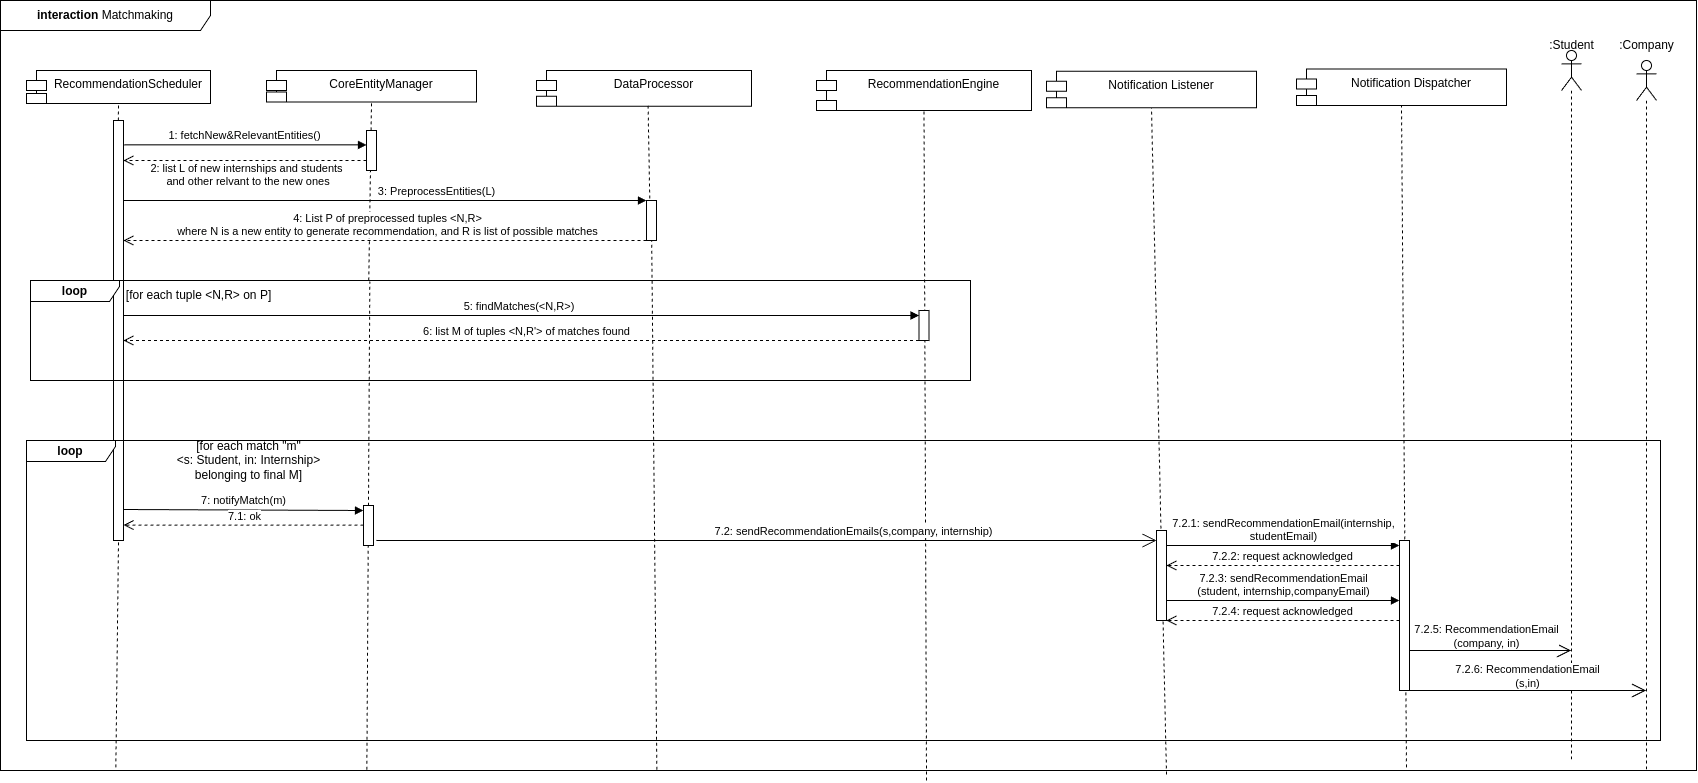
\includegraphics[width=0.9\textheight]{Images/matchmaking-process-sequence.png}
%     }
%     \caption{New Recommendation Sequence Diagram}
%     \label{fig:matchmakingseq}
% \end{figure}

\begin{figure}[H]
\centering
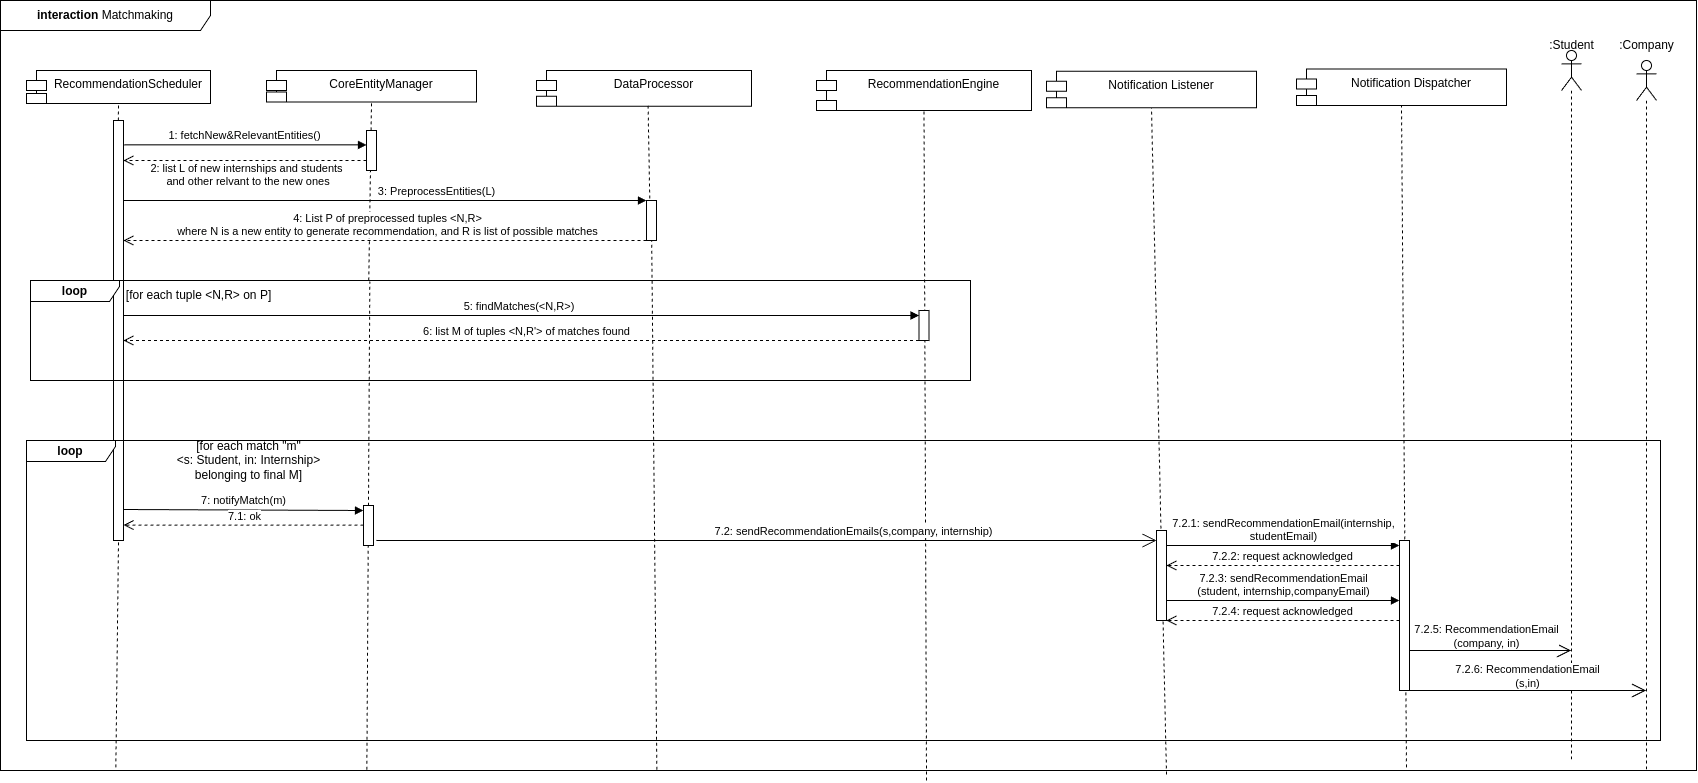
\includegraphics[width=\textwidth]{Images/matchmaking-process-sequence.png}
\caption{\label{fig:matchmakingseq} New Recommendation Sequence Diagram}
\end{figure}

The process begins with the RecommendationScheduler invoking fetchNew\&RelevantEntities() method on the CoreEntityManager (this is scheduled as a CronJob process on the server's OS and is fired regularly). This retrieves a list (L) of newly added internships and students, as well as entities relevant to them according to hard filters (such as the candidate's refusal to move country, for example). 

Once all the new and relevant students and internships are returned to RecommendationScheduler, it calls the DataProcessor to preprocess these entitites. The DataProcessor now generates a structured list P of tuples <N,R> where each N is a new internship or student and R is a list of all relevant counterparts to it. Now, with data structured in a way the RecommendationEngine can understand it, the RecommendationScheduler sends  the tuples one by one to the RecommendationEngine, that returns a list M of tuples of recommended matches based on its internal algorithm.

Now, to send the notifications, for each tuple <N, R> in M, notify the CoreEntity manager through notifcyMatch(n), which in turn will send a message to the NotificationListener, that passes this on to the NotificationDispatcher, which fires all recomenddation emails once they are gathered and its internal algorithm decides to (for example, the company's emails may be buffered until many recommendations are reached, or sent every week, etc.).


\textbf{[UC8] New Internship}

The company employee, already logged in, clicks ``New Internship Position'' on the FrontEndInterface. The FrontEndInterface retrieves the form from the MainPlatform, which displays fields for the internship details (name, requirements, duration, etc.). After the company employee completes and submits the form (included use case: form filling), the MainPlatform passes the new internship information to the CoreEntityManager for storage. Once successfully stored, the CoreEntityManager returns an ``OK'' to the MainPlatform, which confirms with the FrontEndInterface that the position is created. The FrontEndInterface then displays to the company employee that the internship position is now published.

\textbf{[UC9] Cancel Internship}

The company employee, already logged in, opens ``Open Internships'' on the FrontEndInterface. The MainPlatform fetches the list of open internships from the CoreEntityManager, which returns them for display. When the employee chooses an internship to cancel and clicks ``Cancel Internship,'' the FrontEndInterface sends this request to the MainPlatform. The MainPlatform passes the cancellation to the CoreEntityManager, which updates the internship’s state to ``cancelled''. Because of this state change, the internship no longer appears in searches or recommendations. The CoreEntityManager then notifies the MainPlatform, which confirms the cancellation to the FrontEndInterface, displaying to the company's actor that the internship was successfully canceled.

\textbf{[UC10] Schedule Interview} (Figure \ref{fig:schedulesequence})
\begin{figure}[H]
\centering
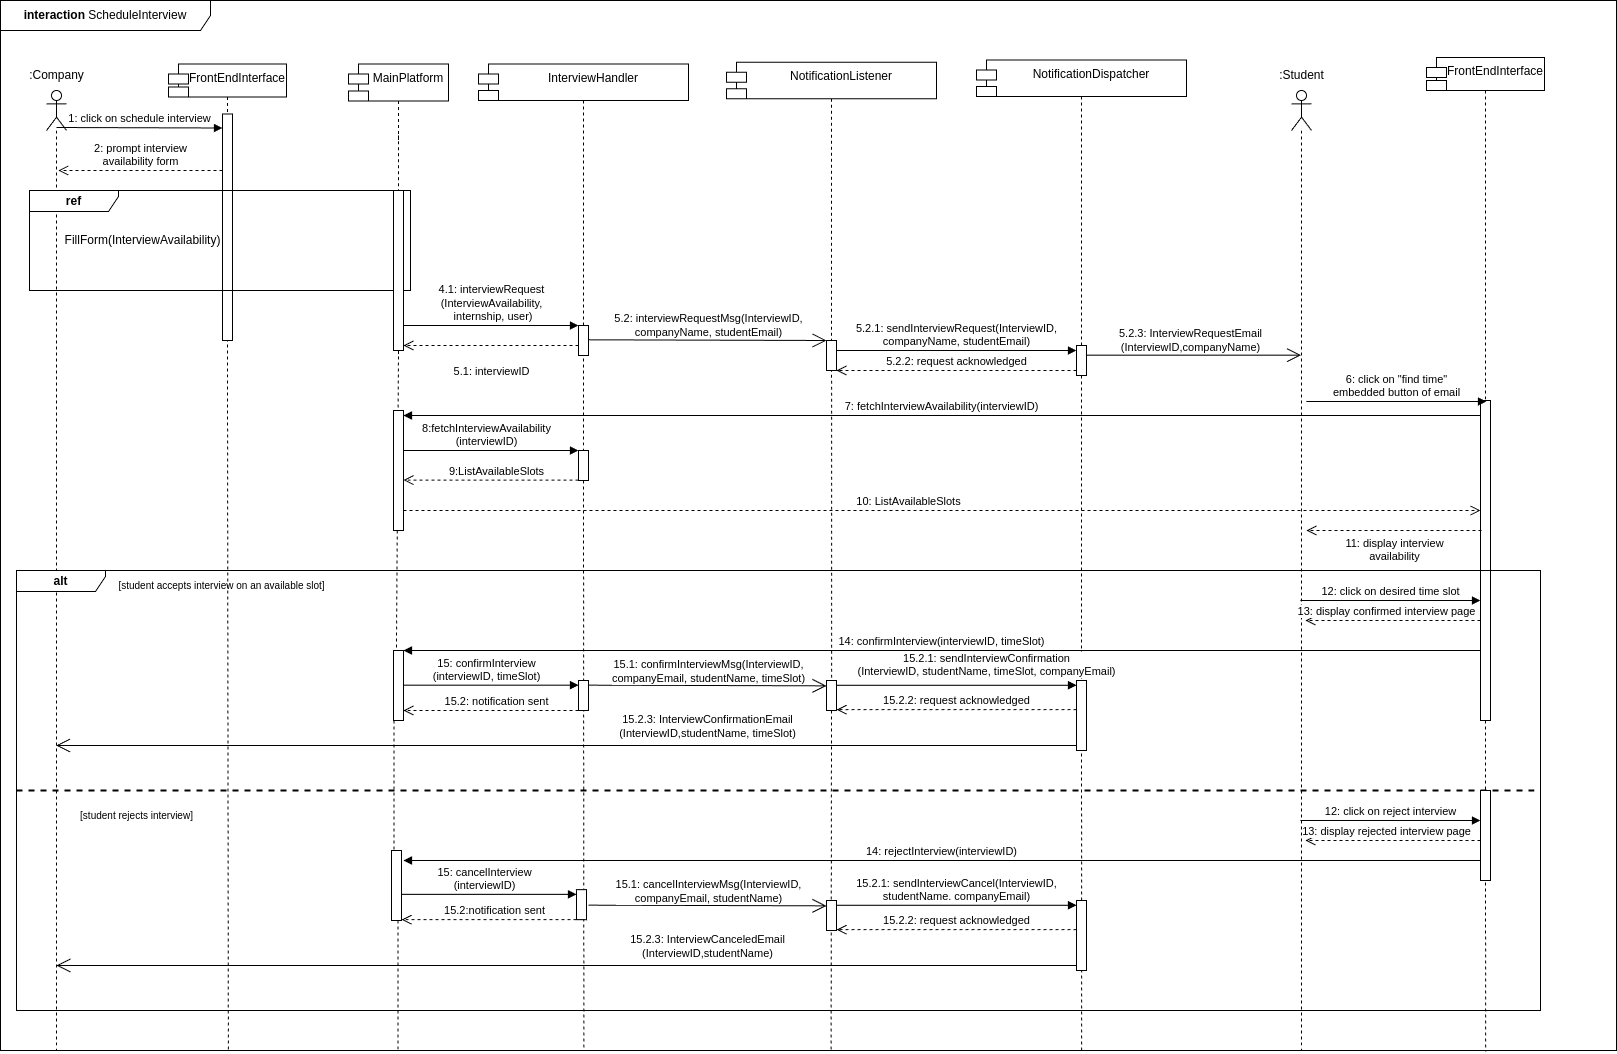
\includegraphics[width=\textwidth]{Images/schedule-interview-sequence.png}
\caption{\label{fig:schedulesequence} Schedule Interview Sequence Diagram}
\end{figure}


The process is started when a Company actor clicks on the "schedule interview" , which makes the FrontEndInterface prompt an availability form for the company agent to fill with the available date and time, the filled answers on the FrontEndInterface are passed to the MainPlatform, that also passes it to the Interview Handler, which creates the interview and returns an ID. This component also starts the notification process sending a message to the NotificationListener, which ends with the Student getting an email.

Once Student clicks on the "find time" button on the email, they are redirected to the S\&C page and another instance of FrontEndInterface starts running on the browser, which fetches the interview availability from the MainPlatform to list the available slots to the Student, which also involves the MainPlatform getting back from the InterviewHandler the availability of the stored interview.

With the availability displayed to the Student, they may either choose a Slot or reject the Interview. In the first case scenario, the FrontEndInterface passes the confirmation to the MainPlatform, which then passes it to the InterviewHandler so the state of the interview is changed and a notification sent to the company's email with a confirmation of date and time for the interview. If, instead, the Student rejects the interview, the same process happens but with rejection messages and the logic inside the InterviewHandler changes.

\textbf{[UC11] Process Interview}
(Figure \ref{fig:processinterviewsequence})
\begin{figure}[H]
\centering
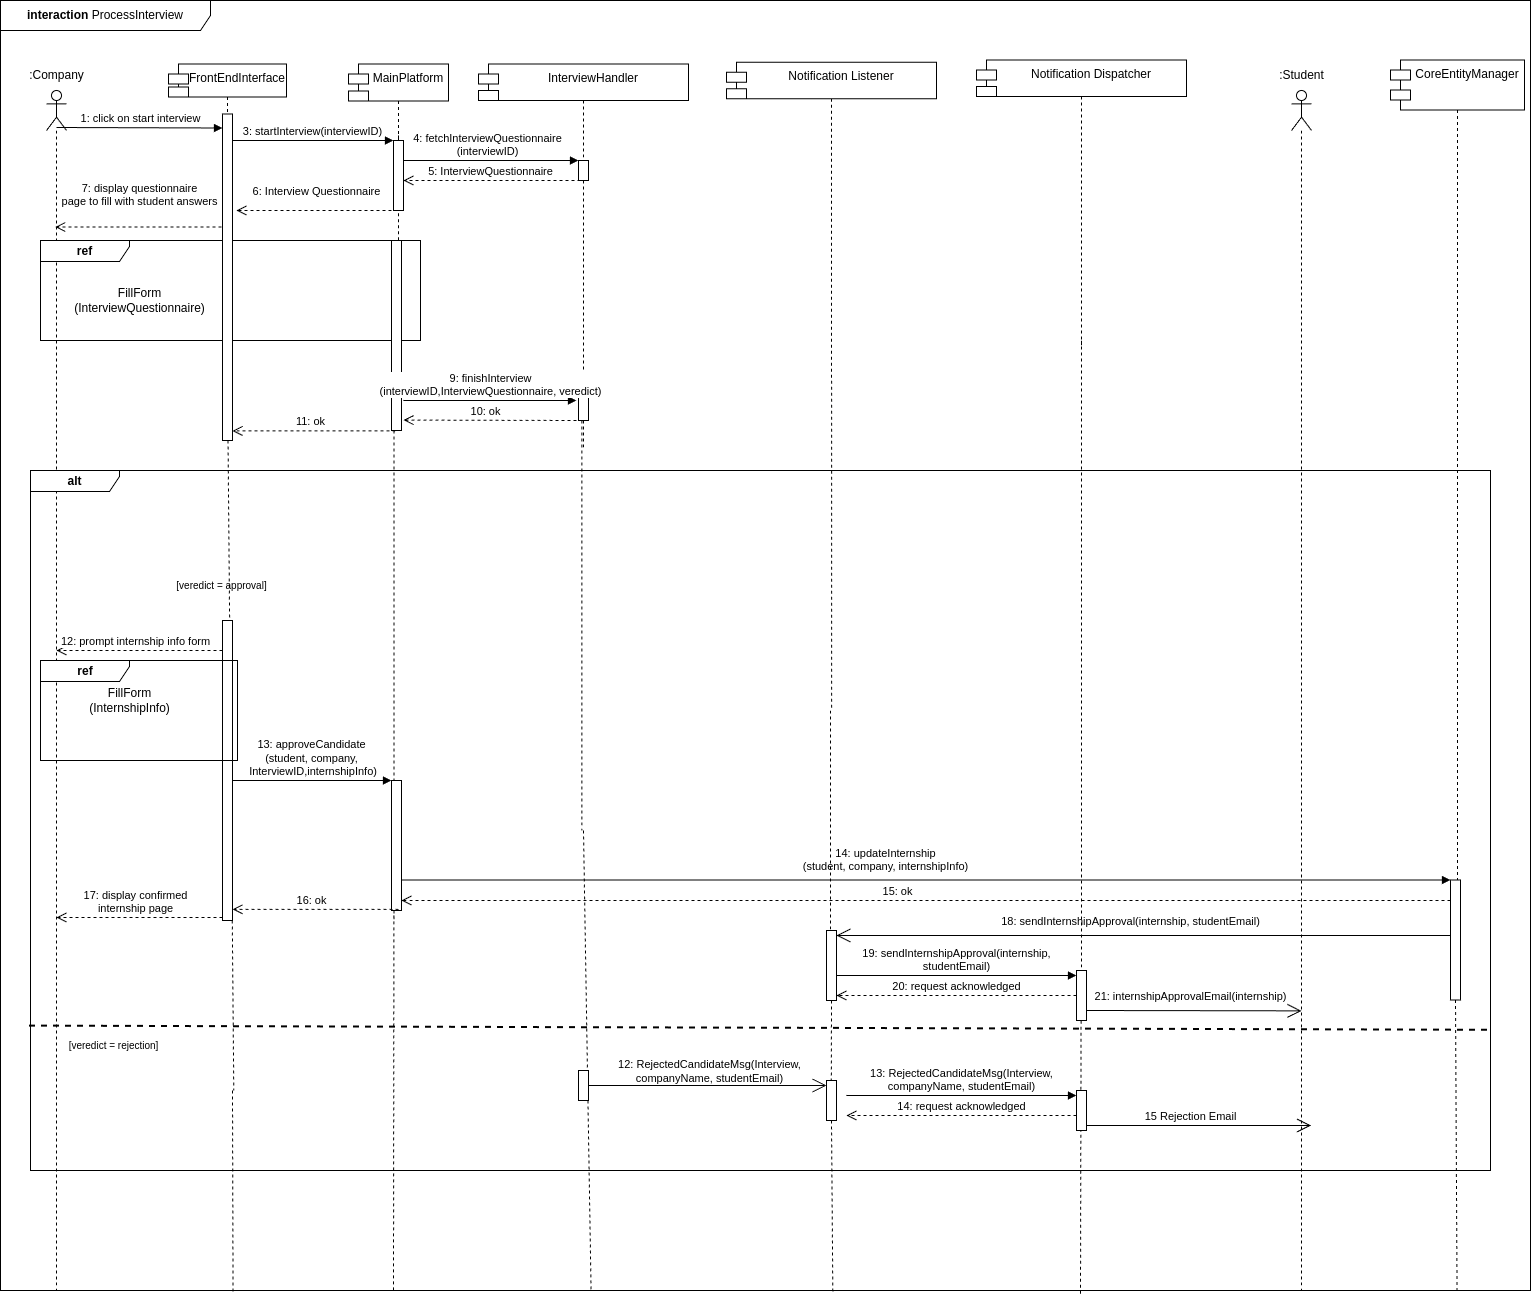
\includegraphics[width=\textwidth]{Images/interview_process-sequence.png}
\caption{\label{fig:processinterviewsequence} Process Interview Sequence Diagram}
\end{figure}

The process is started when a Company actor clicks on the "start interview" , which makes the FrontEndInterface pass this to the MainPlatform as a request for the form to be filled during the interview. The MainPlatform then fetches the form from the InterviewHandler through the interviewID, and the form is passed all the way back to the Company through the display on the FrontEndInterface. Once the form is filled, the interview is finished with a filled form and a veredict, both of which the FrontEndInterface passes to the MainPlatform so it can pass to the InterviewHandler to update the interview status. With the status saved, S\&C proceeds to process the result and notify the student.

If the veredict is true, the FrontEndInterface uses the internship info form (with information wuch as start date, place, etc.) and prompts it to the Company's actor. When it's filled, this component passes the internship information to the CoreEntityManager so it can alter its status and information. Once done with its internal logic, it sends triggers the email notification process by sending a message to the NotificationListener.

In the case of the veredict being false, the only further action needed is to notify the Student since the InterviewHandler already got the veredict and processed it internally, so this component is the one to trigger the notification process by senidng a message to the NotificationListener.


\textbf{[UC12] New Complaint}

The user, already logged in, navigates to ``Ongoing Internships'' on the FrontEndInterface. The FrontEndInterface requests the list of internships from the MainPlatform, which in turn fetches them from the CoreEntityManager and displays them. The user selects the relevant internship and clicks ``Create Complaint,'' triggering the complaint form (included use case: form filling). Once submitted, the FrontEndInterface sends the complaint data to the MainPlatform, which forwards it to the HistoryManager (responsible for feedback, complaints, and analytics). The HistoryManager stores the complaint in the internal database and returns an ``OK'' to the MainPlatform, which confirms success to the FrontEndInterface.


\textbf{[UC13] Post Internship Feedback}

With the user in the ``Provide Feedback'' page of a given closed internship, The FrontEndInterface then displays a feedback form (included use case: form filling). After submission, it sends the feedback data to the MainPlatform, which forwards it to the HistoryManager for storage and calls the CoreEntityManager to update the internship’s status. Finally, the CoreEntityManager triggers a notification handled by the NotificationListener and later passed on to the NotificationDispatcher, alerting the other party (student or company) that the feedback has been submitted.



\section{Component interfaces}

This section introduces every interface of the modeled components, so that the runtime behavior described previously can be understood in a component-level abstraction and to aid the developer on their implementation.

\subsubsection{FrontEndInterface} 


This component offers no interfaces since it is, in itself, a visual interface to the user that interact via web browsing.




\subsubsection{MainPlatform} 

This component offers only one interface, \textbf{ApplicationInterface}
which is offered to the FrontEndInterface:
\begin{itemize}
    \item \texttt{submitForm(formData)} 
    Sends form data from the frontend to be processed.
    \item \texttt{requestStudentRegistration(regData)} Initiates a student registration request.
    \item \texttt{requestCompanyRegistration(regData)} Initiates a company registration request.
    \item \texttt{login(email, password)} Captures user credentials and forwards them for authentication.
    \item \texttt{applyToInternship(internshipId)} Sends the student’s application request for a specific internship.
    \item \texttt{createInternship(data)} Submits new internship details for creation.
    \item \texttt{viewOpenInternships(companyID)} Requests the list of open internships for a given company.
    \item \texttt{cancelInternship(internshipId)}
    \item \texttt{fetchHistory(userID)}
    This is used to fetch the user search history, returning it as a list of performed searches.
    \item \texttt{searchInternship(searchCriteria)}
    This is used to pass the searchCriteria to the CoreEntityManager to perform the search on its database, it returns either a "no results" message or a list of internships to display
    \item \texttt{fetchCompleteInternshipInfo(internshipID)}
    This is used to fetch the complete information about an specific internship (the FrontEndInterface uses it after the User clicks on a specific internship). It returns the internshipInfo.
    \item \texttt{finishInterview(interviewID, interviewQuestionnaire, veredict)}
    This is used so that the FrontEndInterface indicates that the interview with interviewID is finished and the provided information is composed of the filled interviewQuestionnaire and the veredict upon the interview. This is passed on to the interviewHandler and returns just an "ok" message to indicate everything worked out fine.
    \item \texttt{fileComplaint(internshipId, complaint)} Submits a complaint for a specific internship.
    \item \texttt{submitFeedback(internshipId, feedback)} Sends user feedback about a specific internship.
\end{itemize}



\subsubsection{AuthenticationService}

This component offers only one interface, \textbf{UserSession}, which is offered to the MainPlatform:
\begin{itemize}
    \item \texttt{createAccount(email, password)} Creates a new user account.
    \item \texttt{authenticate(email, password)} Validates credentials.
\end{itemize}



\subsubsection{CoreEntityManager}
This component offers two different interfaces.

\textbf{InspectEntities} is offered to the RecommendationScheduler:
\begin{itemize}
    \item \texttt{fetchNewAndRelevantEntities()}
    This is used to fetch all the new entities and the ones relevant to those new ones in terms of matchmaking. It triggers an access to the database, as well as some internal logic to apply the hard filters specified on the newly fetched entities(e.g. a student refusal to move country) to define the "relevant" ones to be searched. It returns a list of found internhsips and students, both new or relevant.
    \item \texttt{notifyMatch(m: <s:Student, in: Internship>)}
    This is used to notify the component that a match has been found between `in` and `s`. This activates the internal match dealing logic of CoreEntityManager and triggers the email-sending process to both parts.
\end{itemize}

\textbf{EntitiesManagement} is offered to the MainPlatform:
\begin{itemize}
    \item \texttt{storeData(formData)} Saves the form data into the internal storage.
    \item \texttt{storeStudentProfile(userID, workProfile)} Stores the student’s work profile information.
    \item \texttt{storeCompanyProfile(userID, compProfile)} Stores the company’s profile information.
    \item \texttt{createApplication(userId: int, internshipId: int)} Logs the application entry into the system.
    \item \texttt{searchInternship(searchCriteria)}
    This inputs the searchCriteria specified by the user and triggers an access to its internal database. It returns a list of found internships
    \item \texttt{storeInternship(data)} Persists the new internship information to storage.
    \item \texttt{fetchInternships(companyID, state?)} Retrieves internships by company and (optionally) state.
    \item \texttt{updateInternshipState(internshipId, newState)} Changes the internship’s state.
\end{itemize}



\subsubsection{InterviewHandler}
This component offers only one interface, \textbf{InterviewManagement}, which is offered to the MainPlatform
\begin{itemize}
    \item \texttt{interviewRequest(interviewAvailability, internship, user)}
    This is used to request a new interview, leading to the instancing of a interview entity and altering the database records. It also triggers a notification message to the Notification Listener so that the Student gets an email about the attemptive interview. It returns the interviewID of the newly instanced interview.
    \item \texttt{fetchInterviewAvailability(interviewID)}
    This is used to consult the availability of an existing interview, instanced through the previous documented call. It returns the interview availability, which is just a list of the available time slots.
    \item \texttt{confirmInterview(interviewID, timeSlot)}
    This is used to confirm an attemptive interview with interviewID in a given timeSlot. Besides internally changing its state, it triggers the notification process by sending a message to NotificationListener so that the Company is notified about the time of the interview. It returns a "notifcation sent" message just meaning everything worked ok.
    \item \texttt{cancelInterview(interviewID)}
    This is used to cancel an attemptive interview with interviewID. Besided internally changing the state of the interview, it sends a message to NotificationListener, so that the Student also gets an email about its cancellation. It also returns a "notifcation sent" message just meaning everything worked ok.
    \item \texttt{fetchInterviewQuestionnaire(interviewID)}
    This is used to get the stored interview questionnaire for the internship corresponding to the interview of interviewID. It returns the requested questionnaire which is only a form.
    \item \texttt{finishInterview(interviewID, interviewQuestionnaire, veredict)}
    This is used to finish an ongoing interview of ID interviewID. It alters the internal state of the interview, saves the provided information and returns an "ok" message to indicate everything worked out fine.
\end{itemize}


\subsubsection{HistoryManager} 

This component offers one interface, \textbf{HistoryFunctions}, which is offered to the Main Platform:
\begin{itemize}
    \item \texttt{saveComplaint(complaint)} Saves the complaint details into the database.
    \item \texttt{saveFeedback(feedback)} Saves the feedback details into the database.
\end{itemize}


\subsubsection{RecommendatonScheduler} 

This component offers no interfaces, since it is only activated regularly through a CronJob scheduled process on its server OS and only uses other interfaces.


\subsubsection{DataProcessor} 

This component offers only one interface, \textbf{PreprocessRecommendationsInterface}, which is offered to the RecommendationScheduler
\begin{itemize}
    \item \texttt{PreprocessEntities(L)} This triggers the component's internal logic of separating the list into tuples <N,R> of new and "relevant to the new" entities, respectively. It returns a list P of such tuples in a format compatible with the RecommendationEngine provided interface ExternalSystemInterface.
\end{itemize}

\subsubsection{RecommendationEngine} 

This component offers only one interface, \textbf{ExternalSystemInterface}, which is offered to the RecommendationScheduler and would depend on the used external system. It is only assumed it can handle one function call to generate matches, and the specific format of input or output can be adjusted on the DataProcessor internals so it is compatible with the used system.
\begin{itemize}
    \item \texttt{findMatches(<N: new entity to generate recommendation for, R: list of relevant entities to N, from which to decide on recommendations>)} This returns a list of tuples <N,R'> of each match found (R' is only one instance of entity, while R is a list).
\end{itemize}

\subsubsection{NotificationListener} 

This component offers only one interface, \textbf{NotifyInterface}, which is used by both InterviewHandler and CoreEntityManager. Each  message only differs in behaviour on the information input, which one of the two entities sends it and which further message is passed on the NotificationDispatcher, to indicate different email formats. They dont't return anything since it is an asynchronous message.
\begin{itemize}
    \item \texttt{interviewRequestMsg(InterviewID, companyName, studentEmail)}
    This is sent by the InterviewManager and triggers a call to sendInterviewRequest()
    \item \texttt{confirmInterviewMsg(InterviewID, companyEmail, studentName, timeSlot)}
    This is sent by the InterviewHandler and triggers a call to sendInterviewConfirmation()
    \item \texttt{cancelInterviewMsg(interviewID, companyEmail, studentName)}
    This is sent by the InterviewHandler and triggers a call to sendInterviewCancel()
    \item \texttt{sendRecommendationEmails(s: Student, company, internship)} This is sent by the CoreEntityManager and triggers two calls to \texttt{sendRecommendationEmail()} to the NotificationDispatcher, one with internship and studentEmail (that will send an email to the student) and the other with the student, internship and companyEmail (that will send an email to the company).
    \item \texttt{RejectedCandidateMsg(Interview, companyName, studentEmail)}
    This is sent by the InterviewHandler and triggers a call to RejectedCandidateMsg() on the NotificationDispatcher interface
    \item \texttt{sendInternshipApproval(internship, studentEmail)}
    This is sent by the CoreEntityManager and triggers a call to sendInternshipApproval() on NotificationDispatches interface
    \item \texttt{sendFeedback(internship, email)}
\end{itemize}


\subsubsection{NotificationDispatcher}
This component offers only one interface, \textbf{EmailDispatchingInterface}, which is offered to the NotificationListener. All function calls on this interface are to request an email to be sent as notification and it always returns a "request acknowledged" message (before the actual email is sent) just to note that the request has arrived properly and the email will be processed. The interface could be defined as only one \texttt{sendEmail(recipient, subject, body)} function, but here it is also specified some of the different forms of emails that may be called from other entities that want a pre-formatted email to be sent without dealing with what that format is.
\begin{itemize}
    \item \texttt{sendEmail(recipient, subject, body)}
    \item \texttt{sendRecommendationEmail(internship,
studentEmail)}
    \item \texttt{sendRecommendationEmail
(student, internship,companyEmail)}
    \item \texttt{sendInterviewRequest(InterviewID,
companyName, studentEmail)}
    \item \texttt{sendInterviewConfirmation(InterviewID,, studentName, timeSlot, companyEmail)}
    \item \texttt{sendInterviewCancel(InterviewID,
 studentName, companyEmail)}
    \item \texttt{sendInternshipApproval(internship,
studentEmail)}
    \item \texttt{RejectedCandidateMsg(Interview,
companyName, studentEmail)}
\end{itemize}


\section{Selected Architectural Styles and Patterns}
\subsection{Microservices Architecture}
The S\&C platform adopts a \textbf{Microservices Architecture} to ensure scalability, modularity, and fault isolation. Each microservice runs in an isolated Docker container, enabling independent development, deployment, and fault isolation. Communication between services is secured using HTTPS, ensuring encrypted data transfer.

\subsection{RecommendationEngine as a Black-Box Component}
The RecommendationEngine is treated as a black-box external component to simplify integration and future updates. With the recent advances in the Artificial Intelligence area, we decided to make minimal assumptions for this component, to facilitate future updates or migrations to other solutions.
For the same reason, we decided to have the DataProcessor as a separate component. This provides flexibility and anticipates changes in the input structure of the RecommendationEngine.

\subsection{Notifications with Asynchronous Communication}
The NotificationListener processes recommendation results asynchronously and passes them to the NotificationDispatcher, which delivers notifications using the sendmail SMTP service. This decoupled setup ensures timely notifications without impacting other system processes.

\subsection{Security Features}
Security measures ensure data protection and system reliability:

\begin{itemize}
    \item \textbf{HTTPS}: Encrypts all communications, safeguarding sensitive data like user credentials and preventing interception or tampering.
    \item \textbf{Firewall}: Positioned between the browser and the load balancer, it protects the system by filtering malicious traffic and enforcing access control.
    \item \textbf{OAuth2 Framework}: The AuthenticationService uses OAuth2, a secure and widely adopted framework, to manage authentication and authorization. This setup ensures user identity verification and secure communication between APIs.
\end{itemize}


\subsection{Distributed Databases with PostgreSQL}
The platform utilizes \textbf{PostgreSQL} in a distributed setup, where each microservice (e.g., \textit{CoreEntityManager}, \textit{InterviewHandler}, \textit{HistoryManager}) has its own dedicated database schema. This design was chosen for its:
\begin{itemize}
    \item \textbf{Decentralization}: Each service manages its own data, aligning with microservices principles and ensuring better fault isolation.
    \item \textbf{Performance}: By distributing data across multiple schemas or databases, query loads are spread out, improving responsiveness.
    \item \textbf{Scalability}: Adding or modifying microservices does not impact the overall system, as each service operates independently on its own database.
\end{itemize}
Data consistency between services is maintained through HTTPS/REST interactions and well-defined APIs.


\section{Other Design Decisions}

\subsection{Preprocessing for Scalability}
In the context of Recommendations, the \textit{CoreEntityManager} microservice preprocesses internship and student datasets before passing them to the \textit{RecommendationHandler}. By filtering data using deterministic rules (e.g., geographical constraints), this design:
\begin{itemize}
    \item Reduces data transfer between components, enhancing system efficiency.
    \item Enables compatibility with external recommendation systems that cannot directly access internal databases.
\end{itemize}

\subsection{Scheduled Recommendations}
The \textit{RecommendationScheduler} periodically initiates the recommendation process using a cron-based system. This ensures:
\begin{itemize}
    \item Timely updates of internship matches for students and companies.
    \item Predictable workloads, optimizing resource utilization across microservices.
\end{itemize}

\subsection{Caching for Enhanced Performance}
The \textit{MainPlatform} component maintains a cache of internship data to minimize interactions with the \textit{CoreEntityManager}. This design decision:
\begin{itemize}
    \item Reduces latency for frequently accessed data.
    \item Ensures efficient use of resources by limiting database queries to only when new or detailed data is required.
\end{itemize}

\subsection{Asynchronous Messaging for Notifications}
The \textit{NotificationListener} uses asynchronous messaging to decouple notification generation from user interactions. Once a recommendation is processed, it triggers the \textit{NotificationDispatcher}, which handles email delivery via the \textit{sendmail SMTP service}. This approach ensures:
\begin{itemize}
    \item Reliable delivery even during peak system usage.
    \item Flexibility in handling multiple notification formats in the future.
\end{itemize}

\subsection{Decentralized Data Storage}
Instead of using a centralized database, the system employs multiple PostgreSQL databases, each dedicated to a specific microservice. This decision:
\begin{itemize}
    \item Enhances modularity by allowing each service to operate independently.
    \item Limits the blast radius of potential failures to individual microservices.
    \item Enables flexibility in scaling individual microservices and their databases based on workload requirements.
\end{itemize}

\subsection{Distributed Deployment}
Each microservice, such as \textit{InterviewHandler}, \textit{HistoryManager}, and \textit{CoreEntityManager}, is independently deployed in Docker containers. This allows:
\begin{itemize}
    \item Horizontal scaling to handle increased traffic.
    \item Simplified maintenance and deployment pipelines.
\end{itemize}

\subsection{Availability and Fault Tolerance}
\subsubsection{Load Balancers}
Load balancers distribute traffic to ensure high availability and prevent server overload:
\begin{itemize}
    \item Between the browser and the CoreApplicationServer, balancing requests to the MainPlatform and AuthenticationService.
    \item Between the CoreApplicationServer and backend servers, routing traffic to the InterviewServer (InterviewHandler) and CoreEntityServer (CoreEntityManager, HistoryManager).
\end{itemize}
This multi-layer approach ensures consistent performance under heavy load.

\subsubsection{Replication Strategy}
Replication enhances availability and performance:
\begin{itemize}
    \item \textbf{Databases}: PostgreSQL’s primary-replica replication ensures data availability and faster reads. Replicas handle frequent queries while the primary handles writes and critical updates.
    \item \textbf{RecommendationEngine}: Replicated on its external cloud platform to ensure uninterrupted service and scalability.
    \item \textbf{Servers}: Core servers are replicated, with load balancers directing traffic for seamless failover in case of hardware or network issues.
   
\end{itemize}

\subsection{System Optimizations}
\subsubsection{Preprocessing}
The DataProcessor applies predefined filters (e.g., geographical constraints) to internship and student datasets before sending them to the RecommendationEngine. This reduces unnecessary processing and improves efficiency.

\subsubsection{Scheduled Recommendations}
The RecommendationScheduler triggers the recommendation process at regular intervals, ensuring timely updates without overloading the system.

\subsubsection{Caching for Performance}
To improve response times, the MainPlatform may cache frequent search results or database interactions based on specific performance metrics. This reduces dependency on direct database queries for common operations.






\chapter{User Interface Design}
\label{ch:user_interface_design}%

\begin{figure}[H]
    \centering
    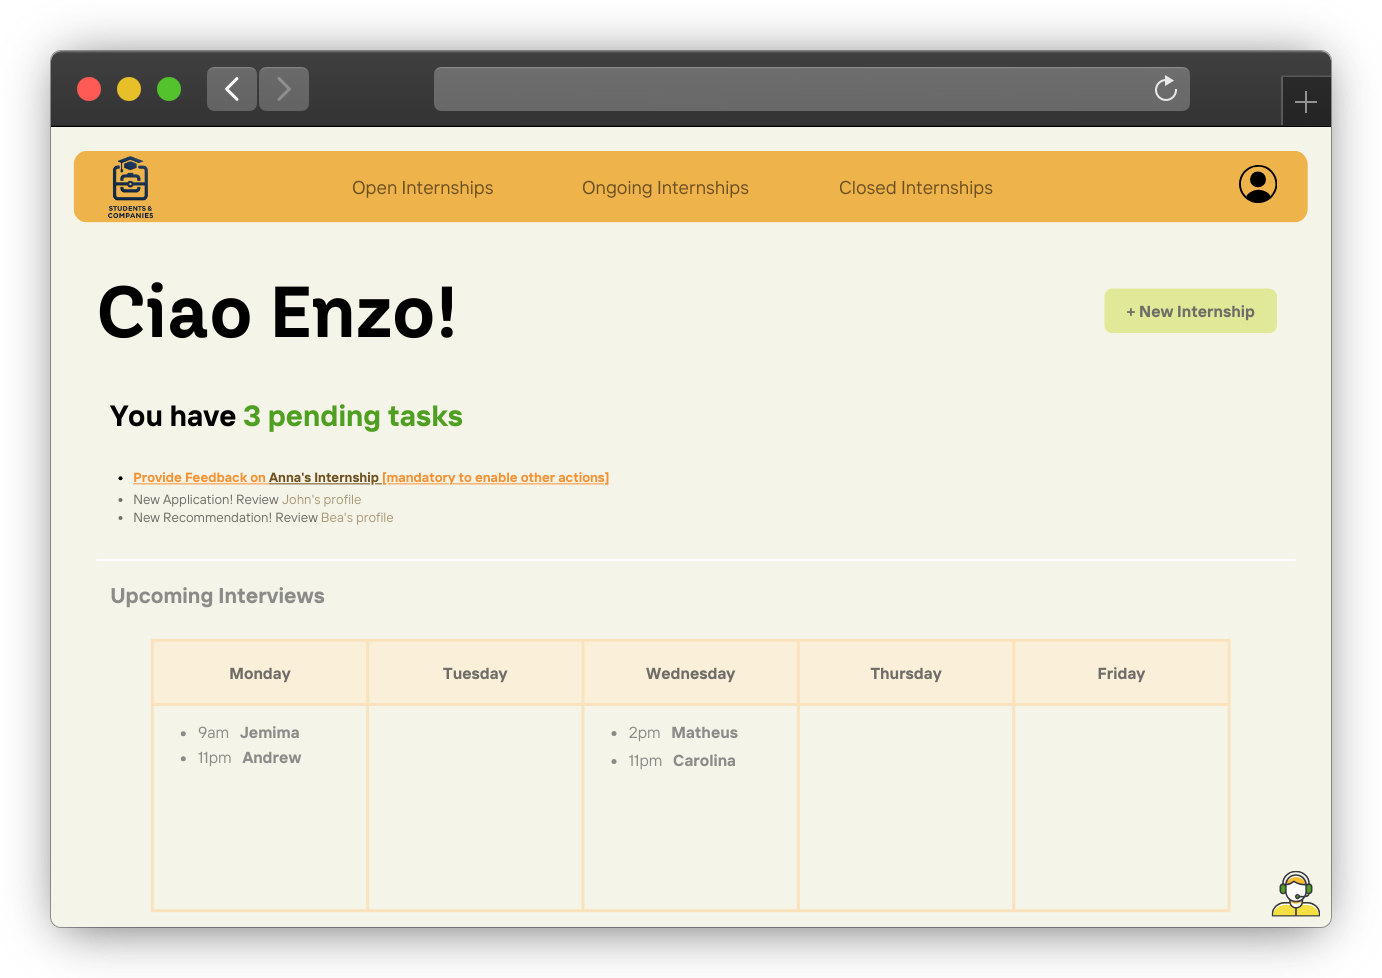
\includegraphics[width=\textwidth]{Images/userInterface-CompanyHomePending.png}
    \caption{Prototype of the Home Page for Company Users, with a pending task}
    \label{fig:CompanyHomePending-user_interface}
\end{figure}


\begin{figure}[H]
    \centering
    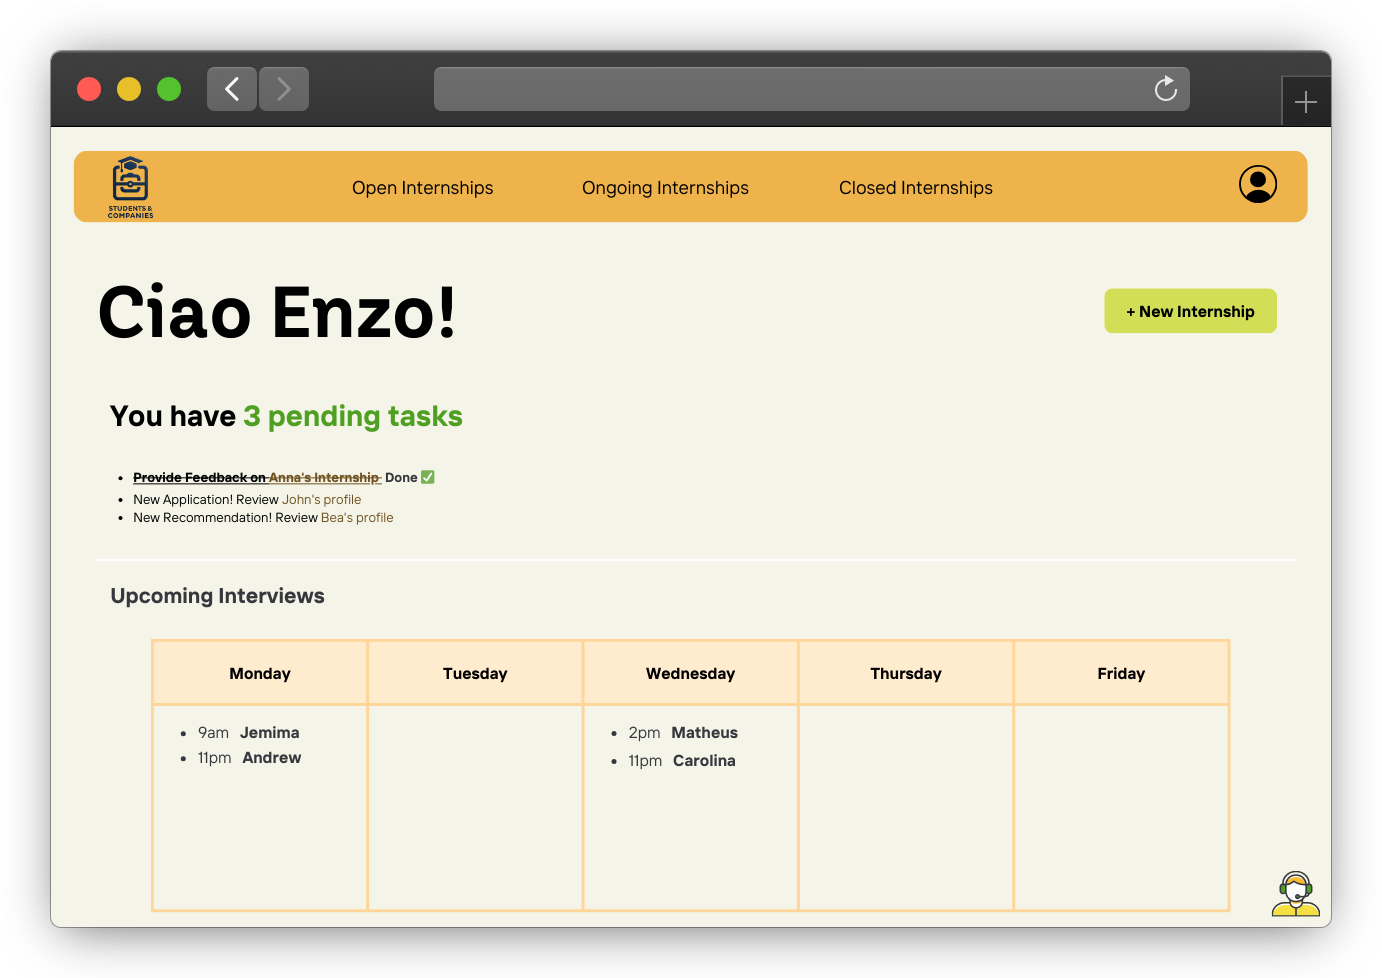
\includegraphics[width=\textwidth]{Images/userInterface-CompanyHomeDone.png}
    \caption{Prototype of the Home Page for Company Users, pending task done}
    \label{fig:CompanyHomeDone-user_interface}
\end{figure}


\begin{figure}[H]
    \centering
    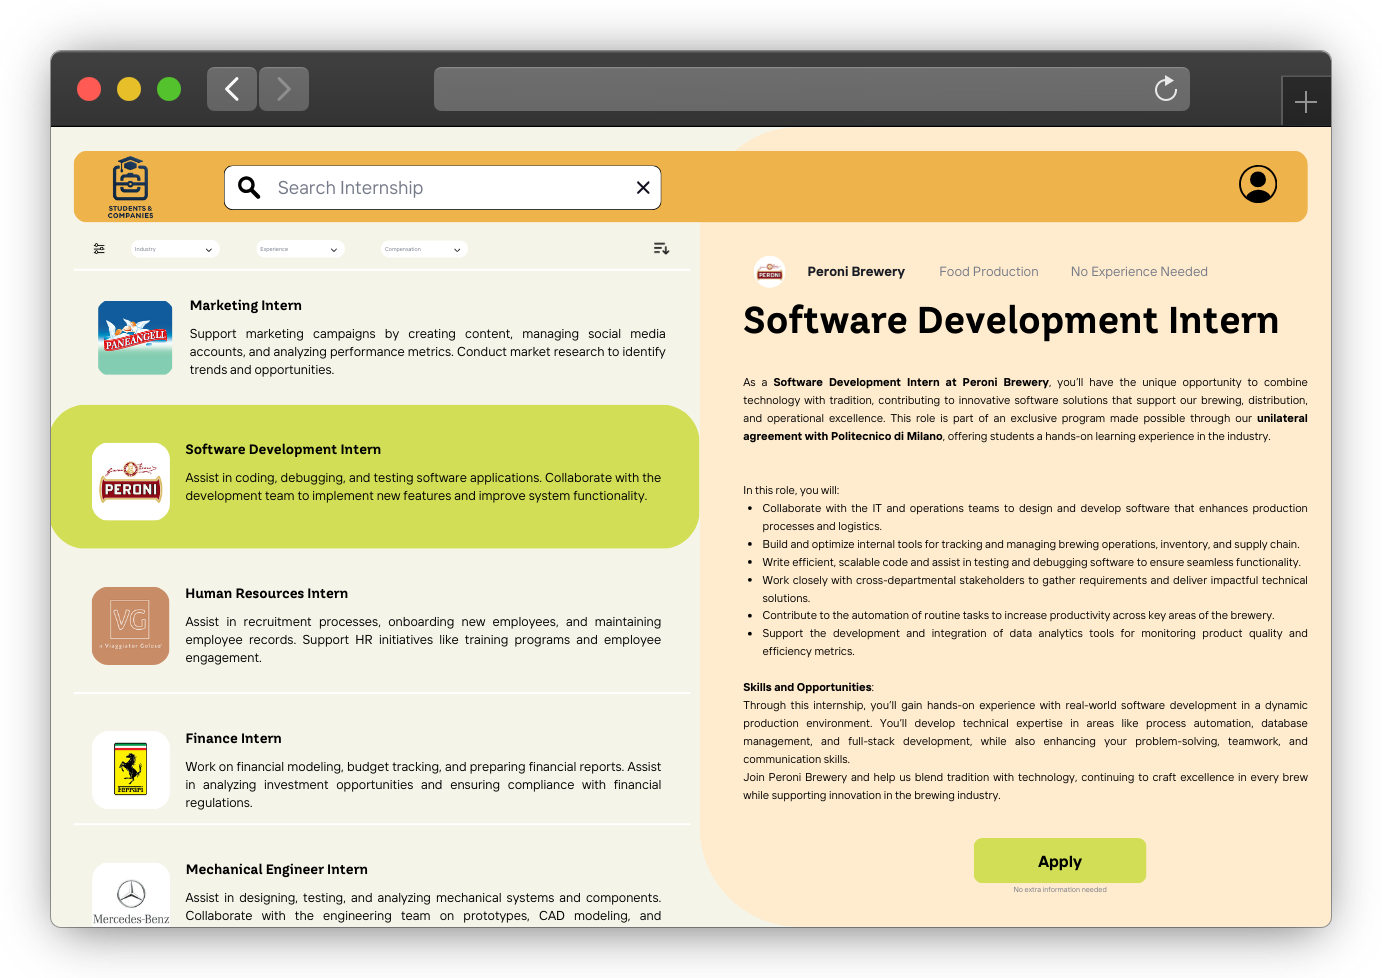
\includegraphics[width=\textwidth]{Images/userInterface-StudentSearch.png}
    \caption{Prototype of the Internship Search (Student)}
    \label{fig:StudentSearch-user_interface}
\end{figure}

\begin{figure}[H]
    \centering
    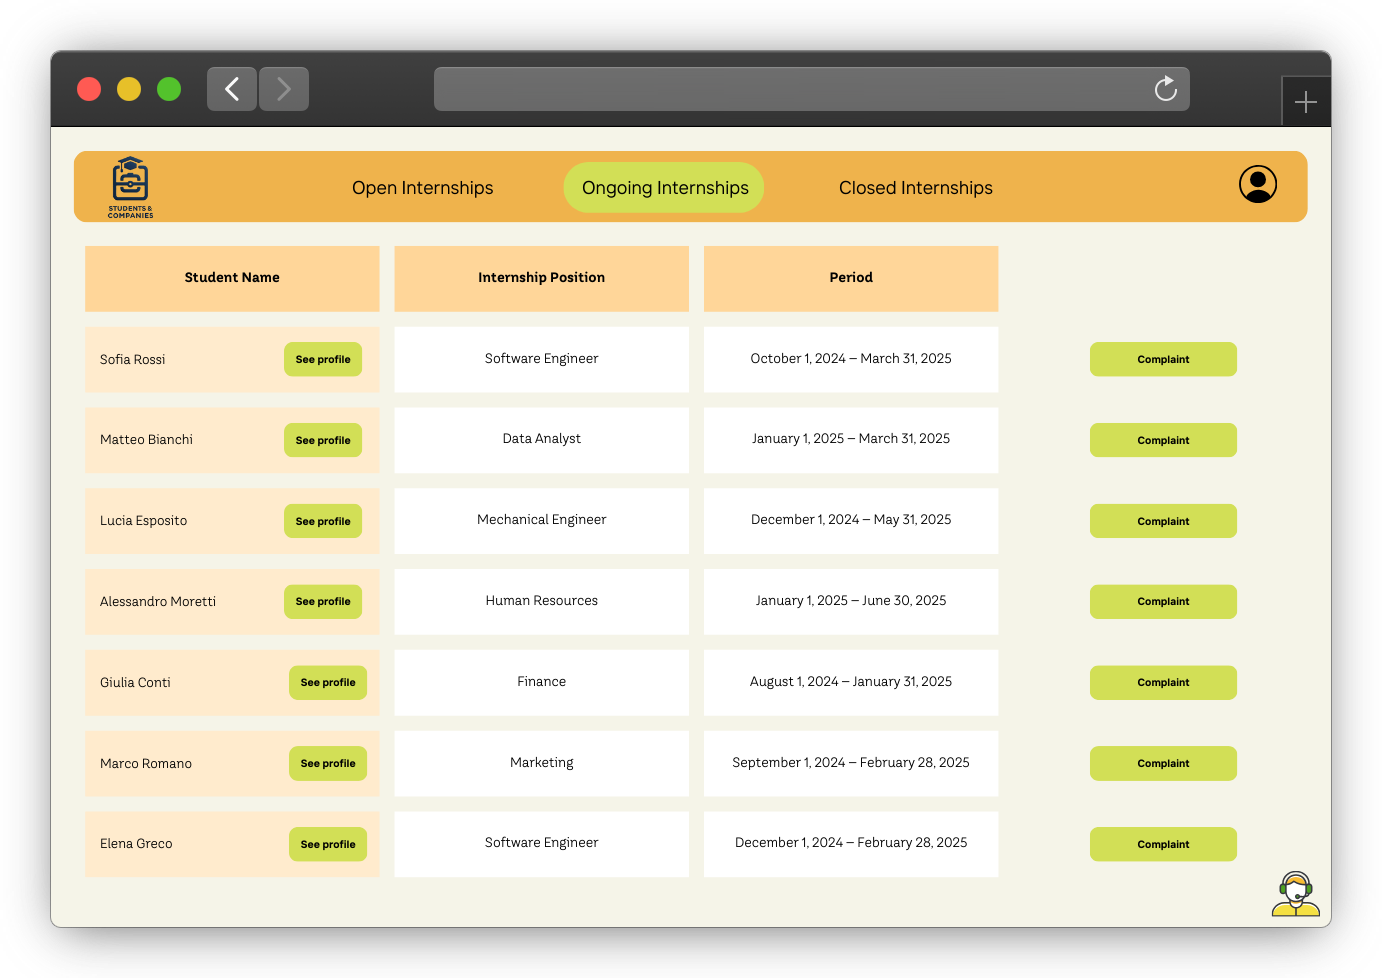
\includegraphics[width=\textwidth]{Images/userInterface-CompanyOngoing.png}
    \caption{Prototype of the Ongoing Internships Tab (Company User)}
    \label{fig:CompanyOngoing-user_interface}
\end{figure}


\chapter{Requirements Traceability}
\label{ch:requirements_traceability}%

In this section it is explained how the requirements defined in the Requirement Analysis and Specification Document, map the design components explained in this document.

\renewcommand{\arraystretch}{1.3}
\begin{longtable}{|p{0.25\textwidth}|p{0.7\textwidth}|}
\caption{\textbf{Sign-Up, Login and Profile Management}} \\ \hline
\multirow{2}{*}{\textbf{Requirements}} & [R1] The system should provide authentication so that each action can be correctly associated with a user \\ 
& [R2] When a student registers the system generates a profile containing their experience, skills, and education \\ \hline
\multirow{4}{*}{\textbf{Components}} 
& AuthenticationService \\ 
& MainPlatform \\ 
& CoreEntityManager \\
& FrontendInterface \\ \hline
\end{longtable}


\renewcommand{\arraystretch}{1.3}
\begin{longtable}{|p{0.25\textwidth}|p{0.7\textwidth}|}
\caption{\textbf{Internship Publication and Management}} \\ \hline
\multirow{4}{*}{\textbf{Requirements}} 
& [R3] The system allows companies to create new internship positions at any time \\ 
& [R4] When a company user clicks on “create internship”, the system prompts the company for all the required information and checks its validity before saving \\ 
& [R5] When an internship is successfully created, the system generates a work profile containing the required experience and skills for the position \\
& [R6] When and internship is successfully created it should be findable through the search internship feature and allow student applications \\
\hline
\multirow{3}{*}{\textbf{Components}} 
& MainPlatform \\ 
& CoreEntityManager \\
& FrontendInterface \\ \hline
\end{longtable}

\renewcommand{\arraystretch}{1.3}
\begin{longtable}{|p{0.25\textwidth}|p{0.7\textwidth}|}
\caption{\textbf{Search and Apply for Internships}} \\ \hline
\multirow{6}{*}{\textbf{Requirements}}
& [R7] When a student searches for an internship through the platform, the system accurately processes the student’s search criteria to display related internships \\
& [R8] When an internship is selected, the system’s user interface summarizes internship information \\
& [R9] When a student searches for an internship through the platform, the displayed internships are within the selected filters \\
& [R10] When a student searches for an internship through the platform, the displayed internships are ordered accordingly to the field specified in student's  criteria \\
& [R11] The system shall allow students to apply to the displayed internship without adding additional information \\
& [R12] When the application button is clicked, the system shall save the student information and profile and notify the company \\
\hline
\multirow{4}{*}{\textbf{Components}} 
& MainPlatform \\ 
& CoreEntityManager \\
& FrontendInterface \\ 
& NotificationHandler Subsystem\\
\hline
\end{longtable}


\renewcommand{\arraystretch}{1.3}
\begin{longtable}{|p{0.25\textwidth}|p{0.7\textwidth}|}
\caption{\textbf{Internship Matching and Recommendation}} \\ \hline
\multirow{4}{*}{\textbf{Requirements}}
& [R13] The system shall provide regular monitoring to all stored profiles from students and internships \\
& [R14] The system shall attempt to match student profiles with internship profiles \\
& [R15] In every match found between an internship and a student, the system shall notify both parts about it \\
& [R16] The matching algorithm used to find recommendations is accurate and can be improved through user feedback \\
\hline
\multirow{4}{*}{\textbf{Components}} 
& RecommendationHandler Subsystem\\
& RecommendationEngine \\
& CoreEntityManager \\
& NotificationHandler Subsystem\\
\hline
\end{longtable}


\renewcommand{\arraystretch}{1.3}
\begin{longtable}{|p{0.25\textwidth}|p{0.7\textwidth}|}
\caption{\textbf{Interview Management and Selection Process}} \\ \hline
\multirow{15}{*}{\textbf{Requirements}} & [R17] The system allows company users to review any student profile \\ 
& [R18] The system allows company users to invite any student to an interview \\ 
& [R19] The system notifies the company when there are new student profiles to review (either applied or recommended) \\  
& [R20] When the company user clicks on “invite to interview” over a student, the system prompts the company user to provide possible availability slots for that specific interview \\  
& [R21] When the company user creates an interview by providing their availability, the system notifies the selected student in less than 6 hours after the interview creation \\  
& [R22] The system allows students to decline the interview they have been invited for \\  
& [R23] If the student does not reply to the interview invitation after 48 hours from the sending time, the system declines the interview automatically \\  
& [R24] When a student accepts an interview invite, the system prompts them to select one of the available time slots for having the interview \\  
& [R25] The system does not allow the student to accept an interview invite without selecting one of the available slots the system provides \\  
& [R26] When the interview starting time comes (slot start), the system provides the company user with the questionnaire associated with the internship the interview is for \\  
& [R27] When the interview finishing time comes (slot end), the system prompts the company user for an interview verdict (approve or reject) \\  
& [R28] When the company user rejects the student after an interview, the system notifies the student \\  
& [R29] When the company user approves the student after an interview, the system prompts them to provide the start time and place of the internship \\  
& [R30] The system does not allow the company to approve the student without providing the internship start time and place \\  
& [R31] When a company user approves the student after an interview, the system notifies the student of the start time and place of the internship \\ \hline
\multirow{5}{*}{\textbf{Components}} 
& FrontendInterface \\  
& MainPlatform \\  
& CoreEntityManager \\  
& NotificationHandler Subsystem\\  
& InterviewHandler \\ \hline
\end{longtable}

\renewcommand{\arraystretch}{1.3}
\begin{longtable}{|p{0.25\textwidth}|p{0.7\textwidth}|}
\caption{\textbf{Feedback and Complaint Management}} \\ \hline
\multirow{5}{*}{\textbf{Requirements}}
& [R32] When the duration time of an internship has passed since its starting time, the system notifies and prompts both the company user and the student to provide feedback on the internship experience \\
& [R33] The system will not allow any user to use other features of the platform (besides login and feedback) when they have pending feedback on past internships \\
& [R34] When a user provides feedback on an internship the system notifies its counterpart in the internship about the received feedback \\
& [R35] The system allows any user to create a complaint about any of their ongoing internships \\
& [R36] When a user creates a complaint the system prompts them to provide a non-empty description of the issue \\
\hline
\multirow{5}{*}{\textbf{Components}} 
& FrontendInterface \\
& MainPlatform \\
& CoreEntityManager \\
& NotificationHandler Subsystem\\
& HistoryManager \\
\hline
\end{longtable}



\chapter{Implementation, Integration and Test Plan}
\label{ch:implementation_integration_and_test_plan}%

\section{Overview}

The system's development and testing will follow a feature-based, bottom-up approach combined with threading. This hybrid strategy ensures systematic integration while making visible progress, leveraging the strengths of both methodologies.

Within each feature thread, the bottom-up strategy is applied by developing and testing the lowest-level components first (e.g., CoreEntityManager in Feature 1) using drivers to simulate higher-level components. Incrementally, higher-level components like MainPlatform are developed and tested with drivers for components such as FrontendInterface. This approach eliminates the need for stubs and facilitates early verification of critical modules, ensuring a stable foundation for higher-level functionality.

Threading complements this by integrating modules that deliver user-visible functionality. It accelerates progress visibility, aligns each thread with specific features (e.g., Internship Matching), and reflects real-world workflows, especially for complex module interactions like NotificationHandler, InterviewHandler, and FrontendInterface.

Together, these strategies create robust building blocks, accelerate feature delivery, and maintain stakeholder confidence. This hybrid approach supports rigorous verification of components and rapid development of user-facing features, aligning with the system’s architecture and requirements \cite{Camilli2024}.

\section{Implementation Plan}

This section specifies the implementation plan.

First, the main features (identified in the Functional Requirements section of the RASD \cite{ContiMarino2024}) are sorted according to the number of components involved (see \hyperref[ch:requirements_traceability]{Requirements Traceability}). However, we do not assume sequential development—features can be developed in parallel by multiple teams to accelerate progress.

\subsubsection{Feature Identification and Sorting}
\begin{enumerate}[label={[F\arabic*]}]
    \item \textbf{Internship Publication and Management} \\ This feature enables companies to publish, manage, and cancel internship opportunities. It includes input verification, ensuring correctness and completeness of internship data. It is prioritized as it involves fewer components, is critical for building the internship database, and is relatively straightforward compared to subsequent features.
    \item \textbf{Search and Apply for Internships} \\ This feature allows students to search and apply for internships using filters like role and location. It includes mechanisms to ensure accurate search results and simple application processes. This comes next as it adds functionality to the published internships, has a moderate number of components, and is critical for student interaction.
    \item \textbf{Internship Matching and Recommendation} \\  This feature leverages external systems to recommend internships to students and suggest suitable candidates to companies. It relies on existing internship and student profiles. It follows as it is more complex, uses more components, and builds upon the foundational features of publication and searching. Also, we hope it acts as a wow-factor for stakeholders.
    \item \textbf{Sign-Up, Login and Profile Management}\\ This feature handles user authentication and profile creation for both students and companies. Profiles include critical data like skills, preferences, and organizational details. This is introduced later as it is less critical initially and involves multiple components.
    \item \textbf{Interview Management and Selection Process} \\ This feature allows scheduling, conducting, and managing interviews. It incorporates availability management and communication via notifications. It is placed here as it is more complex, uses many components, and relies on established profiles, internships, and matchmaking capabilities.
    \item \textbf{Feedback and Complaint Management} \\ This feature facilitates post-internship feedback and complaint filing for ongoing internships. It is implemented last as it is the least critical initially, highly dependent on previous functionalities, and involves a greater number of interactions and components.
\end{enumerate}


\section{Component Integration and Testing}

\subsubsection{[F1] Internship Publication and Management}

\begin{figure}[H]
    \centering
    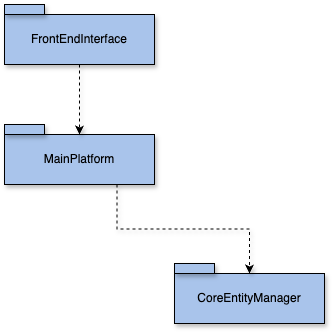
\includegraphics[width=0.5\textwidth]{Images/implementation-testing-hierarchy_f1.png}
    \caption{Components developed in Feature 1}
    \label{fig:implementation_testing_f1}
\end{figure}

The highlighted components in this diagram focus on enabling companies to publish, manage, and cancel internship opportunities. Integration testing involves validating the seamless communication between the FrontEndInterface, MainPlatform, and CoreEntityManager. Tests ensure that input validation, data persistence, and feedback to users function as intended. Mock data is used to simulate internship submissions, and edge cases like missing fields or incorrect formats are checked to confirm the robustness of the feature.

\subsubsection{[F2] Search and Apply for Internships}

\begin{figure}[H]
    \centering
    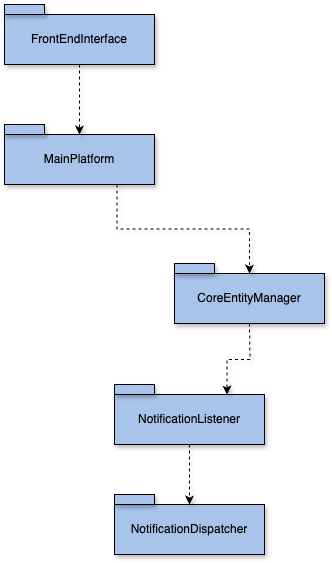
\includegraphics[width=0.5\textwidth]{Images/implementation-testing-hierarchy_f2.png}
    \caption{Components developed in Feature 2}
    \label{fig:implementation_testing_f2}
\end{figure}

The diagram highlights components responsible for retrieving and displaying internships based on user criteria. Testing includes verifying the CoreEntityManager's ability to process search filters and return results efficiently. The interaction between the MainPlatform and the FrontendInterface is tested to confirm accurate display of data. Applying for an internship is tested by ensuring the CoreEntityManager logs applications correctly and triggers appropriate user notifications.


\subsubsection{[F3] Internship Matching and Recommendation}

\begin{figure}[H]
    \centering
    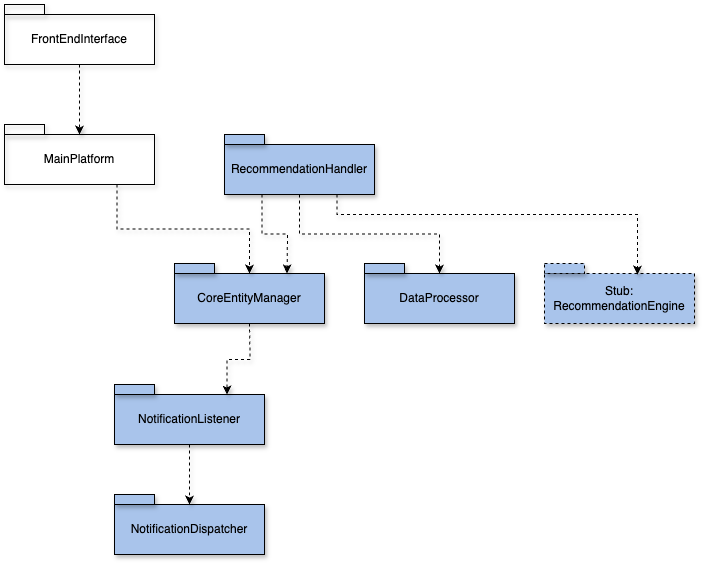
\includegraphics[width=\textwidth]{Images/implementation-testing-hierarchy_f3.png}
    \caption{Components developed in Feature 3}
    \label{fig:implementation_testing_f3}
\end{figure}

This diagram showcases the components involved in recommending internships to students and suggesting candidates to companies. Testing focuses on the integration between the RecommendationScheduler, CoreEntityManager, DataProcessor, and the RecommendationEngine. Tests validate that preprocessing steps filter data accurately and that the external recommendation engine returns valid matches. Notification dispatch for recommendations is tested for timely and correct delivery.

\subsubsection{[F4] Sign-Up, Login and Profile Management}

\begin{figure}[H]
    \centering
    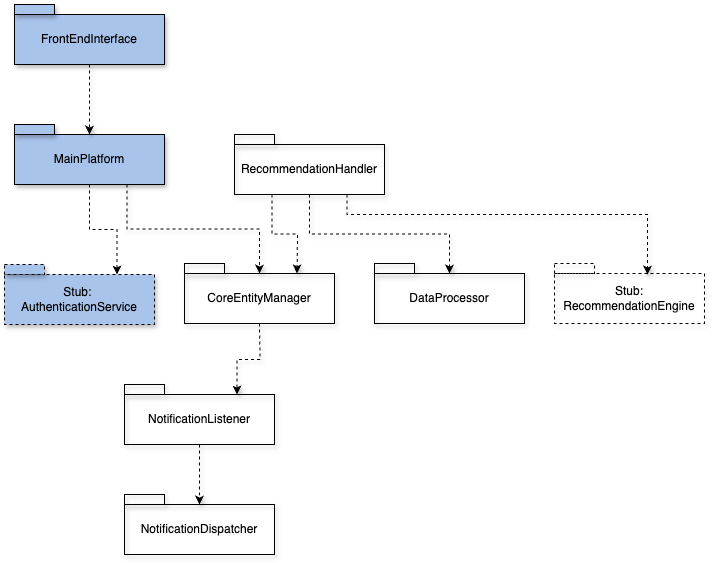
\includegraphics[width=\textwidth]{Images/implementation-testing-hierarchy_f4.png}
    \caption{Components developed in Feature 4}
    \label{fig:implementation_testing_f4}
\end{figure}

The components in this feature enable user registration, authentication, and profile management. Integration tests validate the AuthenticationService for secure handling of user credentials and the CoreEntityManager for storing profile data. Scenarios such as duplicate accounts, incorrect credentials, and partial profile submissions are used to confirm system reliability.

\subsubsection{[F5] Interview Management and Selection Process}

\begin{figure}[H]
    \centering
    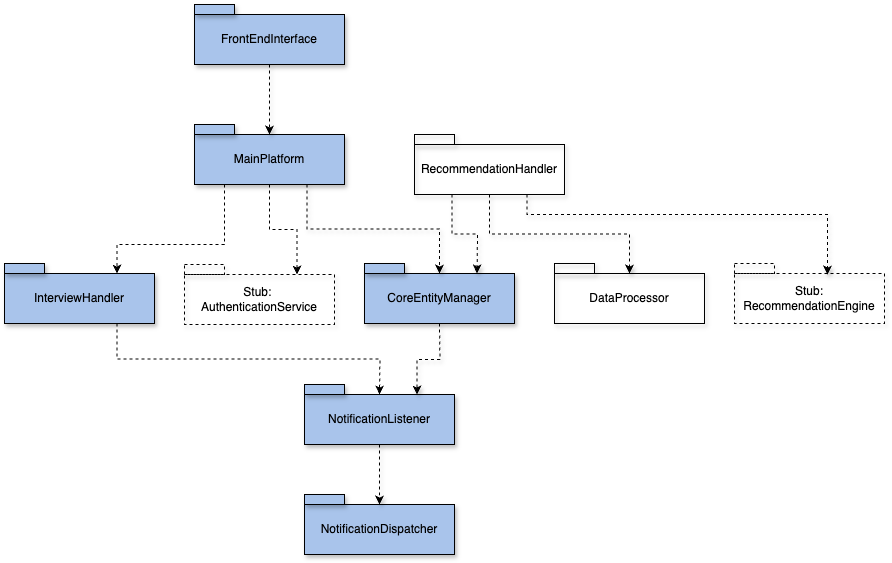
\includegraphics[width=\textwidth]{Images/implementation-testing-hierarchy_f5.png}
    \caption{Components developed in Feature 5}
    \label{fig:implementation_testing_f5}
\end{figure}

The highlighted components manage scheduling, conducting, and updating interviews. Testing ensures proper communication between the FrontendInterface, MainPlatform, and InterviewHandler. Scenarios include creating, confirming, and canceling interviews, with checks for correct notification triggers. The InterviewHandler is also tested for accurately maintaining availability slots and recording outcomes.

\subsubsection{[F6] Feedback and Complaint Management}

\begin{figure}[H]
    \centering
    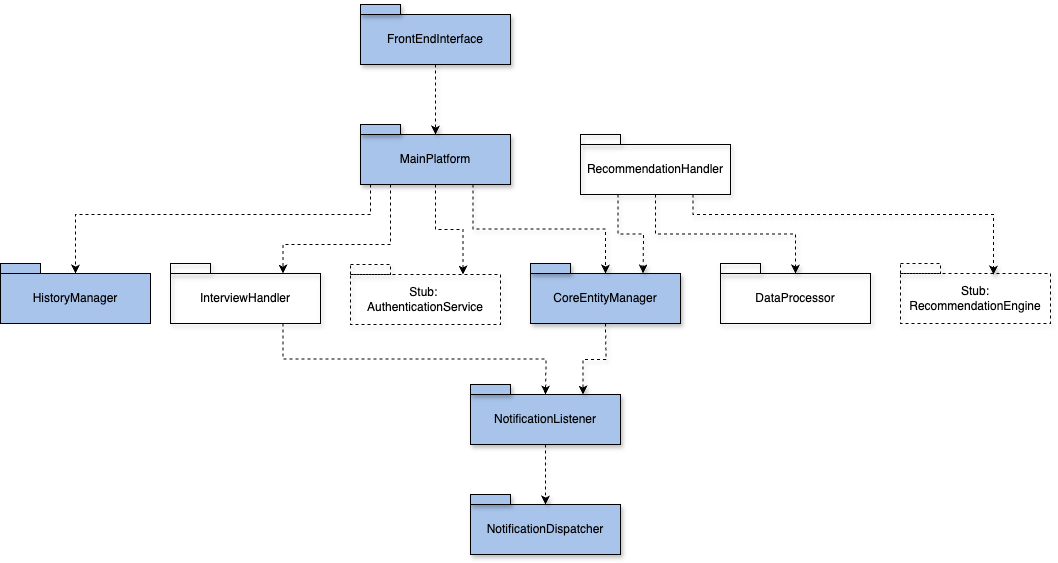
\includegraphics[width=\textwidth]{Images/implementation-testing-hierarchy_f6.png}
    \caption{Components developed in Feature 6}
    \label{fig:implementation_testing_f6}
\end{figure}

This feature integrates components to handle user feedback and complaints. Testing involves ensuring the HistoryManager accurately stores feedback and complaints and that the NotificationListener triggers appropriate alerts. The flow from form submission via the FrontendInterface to data persistence in the CoreEntityManager is validated for reliability and responsiveness.

\section{System Testing}
It is also of uttermost importance that the system is tested is as a whole and not only as separate components, since this complete use  is itself the ultimate goal of a project and the product visible to the user. As mentioned earlier, during the component testing some missing (i.e not yet developed) components may be replaced by stubs and drivers to test the target component. However, even after this test the component must be ensured to work well when integrated with the whole system, which is the purpose of the testing described here.

This means that, once a component is carefully tested as stated before, it can be integrated to the whole platform. Before this new version of the platform is considered an official release, it must undergo additional testing that ensures the fullfilment of the requirements provided on the RASD and not to jeopardize the fullfilment of requirements and behaviour of previous versions or instances of the program.
\subsection{Function Requirements Verification}
Functional Requirements Verification is the first necessary system testing and can be done simply using the software on each use-case and check whether or not it fullfills the specified requirements. The test cases may also be automated so to generate larger and less trivial scenarios corresponding to the specified use cases.
\subsection{Performance Testing}
Performance Testing is useful not only to detect the failure to meet non-functional requirements, but also detect excessively inefficient algorithms and procedures that may lead to bottlenecks on response time, utilization, and throughput. It is also important since, even if a non functional requirement is met on all tested scenarios, the replication and load balancing scheme could lead to a naive use of an inefficient algorithm and, even if it doesnt crash the program, may increase its operation cost. In this phase of testing the workload used is close to expected, and the performance is carefully taken account of to measure a typical usage case.
\subsection{Load Testing}
Load Testing conssits in rising the load from the previous typical usage to identify upper limits of components and subsystems and may lead to architectural changes. The system can be tested with an increased workload until it cannot support or its perfomance metrics become unacceptable. Not only the tested load is increased, but also the testing period, to see how it reacts to increased workloads in larger periods of time, if it balances itself well, if any useless resources remain in use etc. Since this is the sort of testing that can expose memory leaks and buffer overflows, it can also include a layer of fuzziness, in which random inputs are created to see how the system reacts. This is specially useful forthe global interaction of components such as the MainPlatform that have direct access to the FrontEndInterface, but also CoreEntityManager and InterviewHandler that have API calls from the FrontEndInterface through  the MainPlatform (that may not parse the calls appropriately before passing forward, depending on its development - and this would not necessarily be showed by the component testing). Also, the fuzzer can implement a mutation fuzzing from the automated test cases, so to predict common mistakes of the user such as typos or misclicks in certain moments.
\subsection{Stress Testing}
Stress Testing is useful to foresee how the system would react to extreme usage of resources and/or resource crashes - it comprises the matter of failure resistance. In this case, the interfaces can be stressed overwhelming the HTTPS/REST API calls, the replicated components can be diminished and even brought down to zero. Also, the network components can also be subject of stress testing, such as by limiting speeds, and randomly restarting routers. The replicated resources, even if they use open-source frameworks that guarantee some homogeneity, consistency and good replication schemes, can be tested by bringing down essential components randomly, such as the load balancer.
\section{Additional Specification on Testing}
Not only should the system be verified for internal coherence, but it should also be validated for external coherence, that is, to check whether or not it corresponds to the view and demand of users and other stakeholders. To do that, new developed features can go through alpha and beta testing. Once the system verification is done, that version becomes an update - but before being an official release it goes thorugh alpha and beta testing. Alpha testing includes the typical usage with that version of the product by the people directly related to its development, while beta testing opens up to people unrelated to the developed before an official release. 

While this is done to every crucial feature, the specifics and tweaks of every other added eature, for example the email format or the UI page for the recommendation feature, can be added first to target groups to test their experience and feedbacks before becoming a global feature. This takes addvantage of the thread-driven verification to validate parts of whole functionalities and experiences also separately from the whole user group, so to develop a better user experience and understand the users and stakeholders needs while deploying the product.

\chapter{Effort Spent}
\label{ch:effort_spent}%

\begin{table}[H]
    \centering 
    \begin{tabular}{|p{5em} c c |}
    \hline
    \rowcolor{bluepoli!40} % comment this line to remove the color
    \textbf{Activity} & \textbf{Enzo (hours)} & \textbf{María (hours)} \T\B \\
    \hline \hline
    \textbf{Chapter 1} & 5 & 3  \T\B \\
    \textbf{Chapter 2} & 8 & 3  \T\B\\
    \textbf{Chapter 3} & 2 & 3  \B\\
    \textbf{Chapter 4} & 2 & 5  \B\\
    \textbf{Chapter 5} & 3 & 6  \B\\
    \hline
    \end{tabular}
    \\[10pt]
    \caption{Effort spent in hours by each member of the group}
    \label{table:effort_spent}
\end{table}

% %-------------------------------------------------------------------------
% %	BIBLIOGRAPHY
% %-------------------------------------------------------------------------

% \addtocontents{toc}{\vspace{2em}} % Add a gap in the Contents, for aesthetics
\bibliography{bibliography} % The references information are stored in the file named "Thesis_bibliography.bib"

% %-------------------------------------------------------------------------
% %	APPENDICES
% %-------------------------------------------------------------------------

% \cleardoublepage
% \addtocontents{toc}{\vspace{2em}} % Add a gap in the Contents, for aesthetics
% \appendix


% % LIST OF FIGURES
\listoffigures

% % LIST OF TABLES
\listoftables


\cleardoublepage



\end{document}
